% Created 2012-12-19 Wed 11:18
\documentclass[11pt]{article}
\usepackage[utf8]{inputenc}
\usepackage[T1]{fontenc}
\usepackage{fixltx2e}
\usepackage{graphicx}
\usepackage{longtable}
\usepackage{float}
\usepackage{wrapfig}
\usepackage{soul}
\usepackage{textcomp}
\usepackage{marvosym}
\usepackage{wasysym}
\usepackage{latexsym}
\usepackage{amssymb}
\usepackage{hyperref}
\tolerance=1000
\usepackage{ctex}
\usepackage{mathtools}
\everymath{\displaystyle}
\usepackage{libertineotf}
\usepackage{tikz}
\usepackage{algorithm}
\usepackage{algorithmic}
\usepackage{geometry}
\geometry{left=2.5cm, right=2.5cm, top=3cm, bottom=3cm}
\providecommand{\alert}[1]{\textbf{#1}}

\title{\emph{CodeForces solution}}
\author{\emph{罗雨屏}}
\date{\today}
\hypersetup{
  pdfkeywords={},
  pdfsubject={},
  pdfcreator={Emacs Org-mode version 7.8.11}}

\begin{document}

\maketitle

\setcounter{tocdepth}{2}
\tableofcontents
\vspace*{1cm}

\newcommand{\and}{\hspace{0.1cm} \textbf{and} \hspace{0.1cm}}
\newcommand{\xor}{\hspace{0.1cm} \textbf{xor} \hspace{0.1cm}}
\newcommand{\floor}[ 1]{{\lfloor #1 \rfloor}}
\newcommand{\ceil}[ 1]{{\lceil #1 \rceil}}
\newtheorem{improve}{优化}
\newtheorem{theorem}{定理}
\newtheorem{proof}{证明}
\newtheorem{problem}{问题}
\newtheorem{definition}{定义}

\section{Volume I}
\label{sec-1}
\subsection{7E    Defining macros}
\label{sec-1-1}
\subsubsection{题意}
\label{sec-1-1-1}

    给定 C 语言中的若干个宏替换,判断宏是否具有二义性。

    一个宏具有二义性,当且仅当把宏中的内容代入语句后,计算的相对顺序发生了改变。例如 \texttt{sum} 表示 \texttt{x+y} ,则 \texttt{2*sum} 表示的是 \texttt{2*x+y} 。原来应该先计算加法的,现在先计算乘法了,所以是有二义性的。

    $|n| \leq 100$
\subsubsection{算法}
\label{sec-1-1-2}

    考虑建一棵表达式树。对于每个点,他可以表示如下符号:
\begin{enumerate}
\item 一个括号。这种点只能有 1 个孩子,且点的优先级为 $\infty$
\item 加减乘除四则运算中的一个。这种点必须有 2 个孩子,点的优先级依次分别为 1 、 2 、 3、 4
\item 一个变量。这种点没有孩子,优先级为 $\infty$
\end{enumerate}

    由于字符串长度很小,我们可以不用利用栈 $O(n)$ 构造的算法。可以考虑每次扫描一遍当前字符串,求得优先级最低的一个操作,然后以此为根把左右两段的字符串分别递归。
    
    考虑检验一棵子树是否具有二义性。不妨设根节点为 $t$ ,左右孩子分别为 $L, R$ 。如果子树 $t$ 没有二义性,那么子树 $L, R$ 也都没有二义性,且将 $L, R$ 代入 $t$ 进行计算的时候也没有二义性。可以发现,只有 5 种权值。我们建立两个 5x5 的表,分别检验 $t$ 这个操作符是否会影响 $L$ ,以及检验 $t$ 是否会影响 $R$ 。

    剩下的就是细节处理了。

    时间复杂度 $O(n |S|^2)$
\subsection{8D    Two friends}
\label{sec-1-2}
\subsubsection{题意}
\label{sec-1-2-1}

    给定三个点 A, B, C 以及两个参数 $t_1, t_2$ ,要求两条曲线 $C_1$ 和 $C_2$ ,使得:
\begin{enumerate}
\item $C_1, C_2$ 均从 A 开始,到 B 结束。 其中 $C_1$ 必须经过点 C
\item $C_1$ 的长度不超过 $|AC| + |CB| + t_1$
\item $C_2$ 的长度不超过 $|AB| + t_2$
\item $C_1$ 和 $C_2$ 从 A 开始的重合部分长度最大
\end{enumerate}

   输出从 A 开始的最长的重合长度。

   坐标范围不超过 100 。
\subsubsection{算法}
\label{sec-1-2-2}

    一种特殊情况是 $|AB| + t_2 \geq |AC| + |CB|$ ,答案是 $min\{ |AC| + |CB| + t_1, |AB| + t_2\}$ 。

    考虑普通情况。可以知道, $C_2$ 一定不会经过 C ,否则这就为特殊情况了。为了使答案最大,两条曲线一定是直线重合,然后直线走向目标点。可以考虑二分答案。每次二分答案后,我们可以画 3 个圆。如果这三个圆有公共部分,那么就有解,否则就无解。注意一个细节,就是两条曲线可以在一个点附近无限徘徊,所以答案不一定在以 A 为圆心的圆上。
    
    时间复杂度 $O(\log X)$ 。
\subsection{8E    Beads}
\label{sec-1-3}
\subsubsection{题意}
\label{sec-1-3-1}

    定义两个串相等,当且仅当通过把某一个串翻转或反转后两个串相等。

    求所有长度为 $n$ 的且不全为 0 或 1 的串中,所有相等的串中取一个字典序最小的,排序后,第 $k$ 个串。

    $n \leq 50, k \leq 10^{16}$
\subsubsection{算法}
\label{sec-1-3-2}

    这可以看成是一个数位问题。不妨设串前 $\floor{\frac{n}{2}}$ 所代表的二进制数为 $x$ ,后 $\floor{\frac{n}{2}}$ 所代表的二进制数为 $y$ 。考虑这个串为所有和它同构的串中,字典序最小的串的条件。为了描述简洁,我们用 \texttt{\textasciitilde{}x} 表示对于 $x$ 的每一位都按位取反。
\begin{enumerate}
\item 如果 $n$ 为偶数,只要 $x \leq y \and x \leq ~y$ 即可
\item 如果 $n$ 为奇数
\begin{enumerate}
\item 如果中间位为 0 ,要满足 $x \leq y \and x \leq ~y$
\item 如果中间位为 1 ,要满足 $x \leq y \and x < ~y$
\end{enumerate}
\end{enumerate}

    我们可以 $o(1)$ 得到对于一个 $x$ ,存在有多少个合法的 $y$ 。更进一步,可以在 $o(1)$ 的时间内求出所有 $x \leq x^{\prime}$ ,共存在多少个不同的 $y$ 。所以,我们可以二分 $x$ ,求出答案前 $\floor{n}{2}$ 位。

    如果 $n$ 是奇数,我们还有求中间位,这个只要根据中间位为 0 时合法 $y$ 的个数判断即可。

    最后要求后 $\floor{\frac{n}{2}}$ 位。这相当于求把一个区间内的所有的数按照逆序的二进制排序后第 $k$ 个数。我们可以在 $o(1)$ 的时间内得到一个区间内最后一位为 0 或为 1 的数的个数,再与 $k$ 比较一下即可。

    时间复杂度 $O(n^2)$ 。
\subsection{10E   Greedy change}
\label{sec-1-4}
\subsubsection{题意}
\label{sec-1-4-1}

    有 $n$ 种硬币,其价值分别为 $c_i$ ,满足 $\forall i > 1, c_{i - 1} > c_i$ 且 $c_n= 1$ 。现有一种找钱的贪心算法:
\begin{algorithm}
  \label{algo:10E-greedy}
  \caption{求一组硬币,价值和为 $x$}
  \begin{algorithmic}
     \FOR{$i = 1$ to $n$}
        \STATE 找 $\floor{\frac{x}{c_i}}$ 枚价值为 $c_i$ 的硬币
        \STATE $x \leftarrow x \mod{c_i}$
     \ENDFOR
  \end{algorithmic}
\end{algorithm}
    可以发现, \ref{algo:10E-greedy} 并不总是找到硬币数最少的一组解。

    现在的问题是,给定 $c$ ,问最小的一个反例,即 \ref{algo:10E-greedy} 的解不是硬币数最少的解,为多少。如果没有,输出 -1 。

    $n \leq 400$ 。
\subsubsection{算法}
\label{sec-1-4-2}

    我们可以用一个序列 $G(x)$ 表示对于 $x$ ,\ref{algo:10E-greedy} 找到的;用 $M(x)$ 表示硬币数最少的解,也就是最优解。令 $w$ 为最小反例。

    不妨令 $M(w)$ 中第一个非零元素的下标为 $i$ ,最后一个非零元素的下标为 $j$ 显然 $i > 1$ 。可以证明\footnote{参考 《A Polynomial-time Algorithm for the Change-Making Problem》 David Pearson, June 14, 1994 。
 }:
\begin{theorem}
对于每个 $1 \leq k < j$ ,均有 $M(w)[k] = G(c_{i - 1} - 1)[k]$ 。对于每个 $k > j$ ,均有 $M(w)[k] = 0$ 。对于 $k = j$ ,有 $M(w)[k] = G(c_{i - 1} - 1)[k] + 1$ 。
\end{theorem}

    接下来枚举 $i, j$ 即可。每次模拟贪心算法,如果贪心找到的解更劣即可更新答案。

    时间复杂度 $O(n^3)$ 。
\subsection{15E   Triangles}
\label{sec-1-5}
\subsubsection{题意}
\label{sec-1-5-1}

    有一种一个特殊的图,分为 $n$ 层。下图描述了 $n = 12$ 时的图。
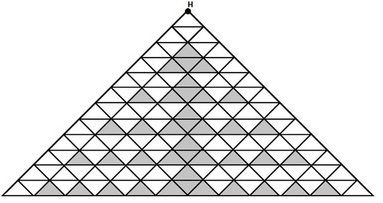
\includegraphics{pic/15E.png}
    现在要求满足以下条件的有向环的个数:
\begin{enumerate}
\item 经过点 H
\item 只沿着黑色边走
\item 经过不止一个点
\item 不经过重复点
\item 不经过灰色方格(原题这么写的,下面为我的解释)
         两个三角形共点称为连通。所有灰色三角形均连通。这条路径不能把灰色三角形分成若干个连通块。
\end{enumerate}

    $n \leq 10^6$
\subsubsection{算法}
\label{sec-1-5-2}

    左右是对称。我们只需求出只走左边到达灰色连通块中最上方的点方案数即可。

    注意到由这个图的特殊性,路径只可能是先沿最左边的边下去,然后沿灰色连通块左边的边上来。这是有拓扑性的。注意到连通块把原图也分成了一棵的样子,树的每个子树是无关的。可以求出子树恰好有 $3x$ 个三角形时,只在子树内部走,从子树最左边的点到达左上方点的方案数。然后用乘法原理即可。

    时间复杂度 $O(N)$ 。
\subsection{17E   Palisection}
\label{sec-1-6}
\subsubsection{题意}
\label{sec-1-6-1}

    给定一个字符串 $s$ ,求所有无序区间对 $(i_1, i_2)$ 的个数,满足:
\begin{enumerate}
\item $s$ 中 $i_1, i_2$ 均为回文串
\item $i_1, i_2$ 有交
\end{enumerate}

   $|s| \leq 10^6$
\subsubsection{算法}
\label{sec-1-6-2}

    首先把原串用扩充,也就是 \texttt{aba} 拓展到 \texttt{\$a\$b\$a\$} 。用 manacher 算法求出以每个点为中心的最长回文串长度 $f_i$ 。接着,考虑如果两个区间有交,我们可以在某个区间的终点统计。现在我们需要统计两个信息:
\begin{enumerate}
\item 每个点成为回文区间左端点的次数 $x_i$
\item 每个点被所有回文区间覆盖的次数 $y_i$
\end{enumerate}

   对于 $x$ ,我们求出 $f_i$ 后,把所有 $[i - f_i, i]$ 内的点的 $x_i$ 加上 1 即可。这可以用差分来维护。对于 $y$ ,我们可以发现差分数组每次需要改动 $O(f_i)$ 个元素,就是在 $i - j + 1$ 处会加 1, $i + j + 1$ 处会减 1 ,其中 $1 \leq j \leq f_i$ 。可以发现每次改动的所有元素是连续的,我们可以考虑维护点,在 $i - f_i + 1$ 处放 + 1 事件,在 $i + 1$ 处放 -2 事件,在 $i + f_i + 1$ 放 + 1 事件。那么这个数组的前缀和的前缀和即为 $y$ 。

   处理 $x$ 和 $y$ 后,枚举对于每个左端点,对答案的贡献是 $\frac{1}{2} y_i (2 x_i - y_i - 1)$ ,累加即可。

   时间复杂度 $O(n)$ 。
\subsection{17C   Balance}
\label{sec-1-7}
\subsubsection{题意}
\label{sec-1-7-1}

    给定一个只含有 \texttt{abc} 的字符串 $S$ ,你每次可以选择两个相邻元素 $i$ 和 $j$ ,并令 $S_i \leftarrow S_j$ 。如果一个字符串中, \texttt{abc} 个数中,任意两个数的差的绝对值不超过 1 ,那么称这个字符串是平衡的。求若干次操作后,所有平衡的字符串的个数。

    $n \leq 150$
\subsubsection{算法}
\label{sec-1-7-2}

    考虑一个字符串 $T$ 。能从 $S$ 经过若干次操作后变成 $T$ 的充要条件是:存在一个长度为 $n$ 的非降正整数序列 $k_i$ ,使得 $S_{k_i} = T_i$ 。

    然后 dp 即可。为了保证每个字符串只被计算一次,我们需要对于每个 $T$ ,都找到一个字典序最小的 $k$ 序列。不妨令 $next[i][c]$ 表示 $S[i:]$ 中,第一个 $c$ 出现的位置。令 $f_{a, b, c, p}$ 表示已经有 $a$ 个 ='a'= , $b$ 个 ='b'= , $c$ 个 ='c'= ,且 $k_{a + b + c} = p$ 的方案数。转移枚举下一个字符是什么,分别转移至 $f_{a + 1, b, c, next[p]['a']}, f_{a, b + 1, c, next[p]['b']}, f_{a, b, c + 1,next[p]['c']}$ 。

    答案在 $f$ 中统计即可。

    时间复杂度 $O(\frac{1}{9}n^4)$
\subsection{19E   Fairy}
\label{sec-1-8}
\subsubsection{题意}
\label{sec-1-8-1}

    给定一个 $n$ 个点 $m$ 条边的图,求出所有的边,使得删掉这些边后的图是二分图。

    $n, m \leq 10^4$
\subsubsection{算法}
\label{sec-1-8-2}

    考虑对原图 dfs 一边,求出 dfs 树。一条边只有被所有的奇环经过的情况下才可能是答案:

    由于我们不可能找出所有的奇环,所以可以考虑一条非树边与一些树边所形成的奇环,不妨称之为单位奇环。我们发现,如果一条边被所有单位奇环经过,且任意偶环均不经过这条边,那么所有的奇环一定经过这条边。因为任意一个奇环均可以通过若干个单位奇环的叠加来表示。如果存在一个奇环不经过这条边,那么这个奇环与若干个奇环的叠加会产生一个经过这条边的偶环,与假设不服。

    所以对于每条边,我们统计有多少条经过这条边的单位奇环,以及是否有偶环经过这条边。这可以通过点事件来实现。对于一条非树边 $u-v$ ,且 
$u$ 深度大于 $v$ 深度,那么在 $u$ 处放一个加一时间, $v$ 处放一个减一事件,那么 $u-v$ 的所有树边的计数器就会加一,就可以统计经过这条边的环的数目。

    时间复杂度 $O(n + m)$ 。
\subsection{23D   Tetragon}
\label{sec-1-9}
\subsubsection{题意}
\label{sec-1-9-1}

    已知一个严格凸的四边形有 3 条边长度相同。给定这三条边的中点坐标,求原凸四边形。不保证有解。 $T$ 组测试数据。

    $T \leq 5 \times 10^4, |X| \leq 10$
\subsubsection{算法}
\label{sec-1-9-2}

    不妨假设连续三条边的中点分别依次为 $A, B, C$ 。我们考虑求出原凸四边形。不妨令 $A, B, C$ 依次为 $t_1 t_2, t_2 t_3, t3_t4$ 的中点。由于这三条边长度相同,可以知道 $t_2$ 一定在 $AB$ 垂直平分线上, $t_3$ 一定在 $BC$ 垂直平分线上。由于 $B$ 为 $t_2 t_3$ 中点,我们可以得到含有 4 个未知数的方程组。通过解这个方程组可以求出 $t_2 t_3$ 两个点。 $t_1 t_4$ 可以由 $t_2 t_3$ 推出来。最后验证多边形是否为凸的即可。

    由于不确定哪条边为中间的边,枚举即可。
    
\section{Volume II}
\label{sec-2}
\subsection{23E   Tree}
\label{sec-2-1}
\subsubsection{题意}
\label{sec-2-1-1}

    给定一棵树,要求删掉若干条边,使得剩下的若干个连通块大小之积最大。

    $n \leq 700$ ,要求高精。
\subsubsection{算法}
\label{sec-2-1-2}

    令 $f_{i, j}$ 表示 $i$ 所在子树, $i$ 所在连通块大小为 $j$ 时,所有不与 $i$ 连通的块的大小之积。我们很容易可以得到一个 dp 。转移的时候用背包加速,枚举是否删除与孩子连接的边以及如果不删的话,孩子所在连通块大小,可以做到复杂度 $O(n^3)$ ,状态 $O(n^2)$ ,转移 $O(n)$ 。

    我们发现,不可能两个大小不小于 2 的连通块发生合并,因为 $\forall x, y \geq 2, xy \geq x + y$ 。所以枚举孩子 $u$ 所在连通块大小的话,我们平摊只要枚举常数个:大小分别为 1、2 ,以及在 $j \leq 2$ 时要枚举 $size[u]$ 个。所以如果不计高精,复杂度为 $O(n^2)$ 。

    由于涉及高精,我选择用 python 编写此题。

    时间复杂度(不计高精): $O(n^2)$
\subsection{26E   Multithreading}
\label{sec-2-2}
\subsubsection{题意}
\label{sec-2-2-1}

    有 $n$ 个进程,每个进程的程序如下:
\begin{algorithm}
  \label{algo:26E}
  \caption{program}
  \begin{algorithmic}
    \FOR{$x = 1$ to $n_i$}
      \STATE $y_i \leftarrow y$
      \STATE $y = y_i + 1$
    \ENDFOR
  \end{algorithmic}
\end{algorithm}
    
    其中 $x$ 是局部变量, $y$ 是全局变量,初始值为 0 。你每次可以允许一个进程执行一条语句。当然每个进程执行语句的顺序是固定的,例如第一个进程的第一个 $y_1 = y$ 必须在第一个 $y = y_1 + 1$ 之前执行。

    问是否存在一种调度顺序,使得所有进程结束后 $y$ 的值为 $W$ 。如果有,输出一组方案。

    $n \leq 100, n_i \leq 10^3, |W| \leq 10^9$ 
\subsubsection{算法}
\label{sec-2-2-2}

    显然是构造。先处理几个特殊情况:
\begin{enumerate}
\item $W < 0$ 或 $W > \sum n_i$ 
         显然无解
\item $W = 1$ 且 $\forall 1 \leq i \leq n, n_i > 1$
         显然也无解
\item $n = 1$ 
         如果 $W = n_1$ ,有且仅有一组解。否则无解。
\end{enumerate}

    可以证明,如果不满足以上任意一组情况,必定有解。

    我们发现,如果一个进程一个进程地执行,那么答案为 $\sum n_i$ 。$y$ 可能比 $W$ 大,我们需要浪费若干个操作。可以发现以下序列可以浪费恰好 2 次对 \texttt{b} 的操作: \texttt{abbbba} 

    于是用同样的思路,我们一开始用某个进程 $z$ 把 $y$ 备份起来,然后不断地浪费其它进程的操作,直到恰好等于答案为止。但是这样还有一种特殊情况,就是把其它进程的操作全部浪费了 $y$ 都比 $W$ 大。我们必须先浪费一部分 \texttt{z} 的操作,而这可以通过另外一个进程来实现。所以流程如下:
\begin{enumerate}
\item 任选一个 $z$
\item 如果有必要,先浪费 $z$ 的操作
\item 不断浪费其它进程的操作
\item 不再浪费,顺序输出剩下操作
\end{enumerate}

    时间复杂度 $O(\sum n_i)$ 。
\subsection{28D   Do not fear, DravDe is kind}
\label{sec-2-3}
\subsubsection{题意}
\label{sec-2-3-1}

    有一个长度为 $n$ 的序列,每个元素有 4 个参数 $v, c, l, r$ 。要求选择一个集合 $S$ ,使得:
\begin{enumerate}
\item $\forall i \in S$ ,满足 $\sum_{j < i, j \in S} c_j = l_i$ 且 $\sum_{j > i, j \in S} c_j = r_i$
\item $\sum_{i \in S} v_i$ 最大
\end{enumerate}
 
    $n \leq 10^5, v, c, l, r \leq 10^5$
\subsubsection{算法}
\label{sec-2-3-2}

    易知, $\forall i \in S$ , $l_i + c_i + r_i$ 是相同的。我们只需把 $l_i + c_i + r_i$ 相同的一起处理即可。

    进一步可以发现, 如果 $i \in S$ , 那么对于最小的比 $i$ 大的 $j$ ,存在 $l_j = l_i + c_i, r_i = r_j + c_j$ 。这事实上是确定了 $i$ 的后继。我们可以实时维护一个 map ,存储 $(l_i + c_i, r_i)$ 相同的时候, $\sum c_i$ 的最大值。求出 $i$ 的值之后,再更新 map 即可。

    时间复杂度 $O(n \log n)$
\subsection{30D   Kings Problem?}
\label{sec-2-4}
\subsubsection{题意}
\label{sec-2-4-1}

    给定 $x$ 轴上 $n$ 个点以及另外一个点 $(x_{n + 1}, y_{n + 1})$ ,求从给定的第 $k$ 个点开始的最小哈密尔顿路径长度。
\subsubsection{算法}
\label{sec-2-4-2}

    如果 $k = n + 1$ ,最优路径一定是先到达最左边或最右边的点,然后按 $x$ 递增或递减的顺序访问所有的点。

    如果 $k \leq n$ ,可以证明最优路径在到达点 $n + 1$ 之前,只可能是下面几种路径之一:
\begin{enumerate}
\item 先到达点 $1$ ,然后到达点 $t$ ,再到达点 $n + 1$
\item 先到达点 $n$ ,然后到达点 $t$ ,再到达点 $n + 1$
\item 先到达点 $t$ ,然后到达点 $1$ ,再到达点 $n + 1$
\item 先到达点 $t$ ,然后到达点 $n$ ,再到达点 $n + 1$
\end{enumerate}

   枚举是哪种情况,再枚举 $t$ ,取最小值即可。
\subsection{30E   Tricky and Clever Password}
\label{sec-2-5}
\subsubsection{题意}
\label{sec-2-5-1}

    给定一个字符串 $S$ ,要求表示成 $A + prefix + B + middle + C + suffix$ 的形式,其中除 middle 外的其余字符串均可以为空,且 prefix 和 suffix 对称相同, middle 为回文串,且 $|prefix + middle + suffix|$ 最大。

    $|S| \leq 10^5$
\subsubsection{算法}
\label{sec-2-5-2}

    不妨令 $T$ 为 $S$ 翻转后的串。可以知道 prefix 一定是 $T$ 的前缀。我们先用 Manacher 算法用 $O(n)$ 的时间处理出以 $i$ 为中心的最长回文串的长度。考虑枚举 middle 的终点。显然 middle 应该越长越好。那么 prefix 的最长的长度为 middle 之前串中,最长的一个子串,使得这个子串是 $T$ 的前缀,且不能超过 middle 后串的长度。我们用 KMP 算法可以求出 $S$ 的每个前缀 $pre_i$ 的最长后缀,使得这个后缀是 $T$ 的子串。枚举了 middle 的长度后, prefix 的长度显然就是前若干个前缀中最长后缀的最大值,直接求一个前缀最小值即可。

    复杂度 $O(N)$ 。
\subsection{32E   Hide-and-Seek}
\label{sec-2-6}
\subsubsection{题意}
\label{sec-2-6-1}

    给定两个点 V 、P 以及两条线段 M 、 W ,其中 M 表示镜子, W 表示墙。镜子可以反射光线,遵循反射定律。问从 V 点是否可以看到 P 点。

    坐标范围不超过 $10^4$ 。
\subsubsection{算法}
\label{sec-2-6-2}

    从 V 可以看到 P 有两种情况:
\begin{enumerate}
\item V 直接看到 P
         只要求 VP 与 M 、 W 都不相交即可。
\item V 通过镜子反射看到 P
         令 R 为 P 关于 M 的对称点。易知 RV 与 M 有交,令交点为 x ,则 Px、Vx 与 W 无交。
\end{enumerate}

    分别判断即可。细节很多,注意判断 4 点共线的情况。

    时间复杂度 $O(1)$ ,常数较大。
\subsection{35E   Parade}
\label{sec-2-7}
\subsubsection{题意}
\label{sec-2-7-1}

    给定若干个边与坐标轴平行的矩形,且底边在 $x$ 轴上,输出这若干个矩形的并。

    $n \leq 10^5$ ,坐标范围绝对值不超过 $10^9$ 。
\subsubsection{算法}
\label{sec-2-7-2}

    扫描线算法。维护一个多重集合,一个矩形扫描到左端点的时候把它顶边加入集合,扫描到右端点的时候从集合中删除,集合里的最大值就是多边形中,当前 $x$ 坐标下的 $y$ 最大点的 $y$ 。维护集合最大值即可。

    可以用 mulitset 来维护。

    时间复杂度 $O(n \log n)$ 。
\subsection{36E   Two paths}
\label{sec-2-8}
\subsubsection{题意}
\label{sec-2-8-1}

    给定一个图,要求两条欧拉路径,使得每条边在且仅在一条路径中出现。输出方案。

    $m \leq 10^4$
\subsubsection{算法}
\label{sec-2-8-2}

    首先,我们把原图中所有度数为奇数的点配对,每对点都连一条边,重新构一个图,使得新图任意一点的度数均为偶数。

    对于新图的任意一个连通块,我们知道一定存在一条欧拉回路。假设我们共加了 $k$ 条边,则把这 $k$ 条边删掉后一条回路会变成 $k$ 条路径,而且这 $k$ 条路径一定把这个连通块的边全部覆盖了。而且我们知道,如果一个连通块如果存在 $2k$ 个度数为奇数的点,那么至少要 $k$ 条路径才能覆盖完这些边。也就是说,把这些边删掉后,求得的路径覆盖一定是最少的。

    所以我们求出新图的若干条回路后,再把新加的边删掉。如果存在超过 2 条路径或者 $m = 1$ ,显然无解。如果只有 1 条路径,把这条路径拆成两条即可。

    时间复杂度 $O(m)$ 。
\subsection{37E   Trial for Chief}
\label{sec-2-9}
\subsubsection{题意}
\label{sec-2-9-1}

    一个 $n \times m$ 的棋盘,初始全部为白色。你每次可以操作一个 4 连通块(不要求同色),把这个连通块内的所有格子的颜色改为黑色或白色。求把棋盘变为目标状态的最小操作步数。
\subsubsection{算法}
\label{sec-2-9-2}

    建立一个网格图:
\begin{enumerate}
\item 图的每个点代表棋盘的一个格子
\item 如果两个格子相邻,那么对应的两个点会有一条边
\begin{enumerate}
\item 如果两个格子颜色相同,那么边权为 0
\item 否则边权为 1
\end{enumerate}
\end{enumerate}

    可以证明,从任意一个格子出发,最远的黑色格子的距离加上出发点是否为黑色,这个值是恰好从这个格子开始,把整个棋盘染色的最小步数。我们枚举初始点,暴力 SPFA 求最短路即可。

    具体可以参考 2012 年钟沛林集训队互测题目《黑白染色》。
\section{Volume III}
\label{sec-3}
\subsection{39C   Moon Craters}
\label{sec-3-1}
\subsubsection{题意}
\label{sec-3-1-1}

    平面上有 $n$ 个圆,每个圆心的坐标为 $(x_i, 0)$ ,半径为 $r_i$ 。要求选出尽量多的圆,使得选出的圆中,任意两个圆不相交。允许相切。要求输出方案。

    $n \leq 2000$ ,坐标范围绝对值不超过 $10^9$ 。
\subsubsection{算法}
\label{sec-3-1-2}

    我们把圆全部投影到 $x$ 轴上去,可以把原题转化成:选若干条线段,要么不相交,要么包含或在端点相交。显然,点的个数为 $O(n)$ 级。我们把不同的 $x$ 坐标全部离散化掉。

    令 $f_{i, j}$ 表示要求选的线段的所有端点的坐标在 $[i, j]$ 之间,最多选多少条线段。我们可以得到一个 $O(n^2)$ 的 dp :
\begin{enumerate}
\item 如果左端点不在最外层的某条线段中,则最优解为 $f_{i + 1, j}$
\item 否则,枚举这条线段的右端点 $t$ ,要求存在一条线段 $i \to t$ ,此时的最优解为 $f_{i, t} + f_{t, j} + 1$ 。
\end{enumerate}

    由于一条线段 $x \to y$ 当且仅当 $i = x, j \geq y$ 时才会被枚举到,所以总枚举量为 $O(n^2)$ 。

    至于输出方案,我们只需在最后记录最优解来自于第一种转移,还是第二种转移的 $t$ 即可。
\subsection{39A   C*++ Calculations}
\label{sec-3-2}
\subsubsection{题意}
\label{sec-3-2-1}

    给定一个表达式字符串,语法规则如下:
\begin{enumerate}
\item expression ::= summand | expression + summand | expression - summand
\item summand ::= increment | coefficient*increment
\item increment ::= a++ | ++a
\item coefficient ::= 0|1|2|\ldots{}|1000
\end{enumerate}

    给定 $a$ 的初始值,你每次可以计算一个 summand 的值,并且 $a$ 的值会随之改变。

    求一个使得 expression 的值最大的 summand 的计算方案。

    初始时 $|a| \leq 10^3$ , summand 的数目不超过 1000 。
\subsubsection{算法}
\label{sec-3-2-2}

    首先我们把 expression 拆成若干个 summand ,每个 summand 用一个二元组 $(coef, inc)$ 来表示,其中 $coef$ 指带符号的 increment 的系数, $inc$ 指这个 summand 是 a++ 还是 ++a 。

    可以证明:
\begin{theorem}
   每次计算 $coef$ 最小的一个 summand 会使得答案最优。
\end{theorem}

    考虑最优解中连续两个 summand : $(coef_1, inc_1)$ 和 $(coef_2, inc_2)$ 。如果先计算第一个,得到的值是 $a(coef_1 + inc_1) + (coef_2 + inc_2) (a + 1)$ ;先计算第二个,得到的值是 $a(coef_2 + inc_2) + (coef_1 + inc_1) (a + 1)$ 。两式相减,得到 $coef_1 < coef_2$ 时,先计算第一个会使得答案更大。

    排序后模拟即可。

    时间复杂度 $O(summand)$ 。
\subsection{39E   What Has Dirichlet Got to Do with That?}
\label{sec-3-3}
\subsubsection{题意}
\label{sec-3-3-1}

    有两个数 $a, b$ 。两人博弈,每人轮流操作,每次需要给 $a$ 或 $b$ 加上 1 ,如果先手操作后 $a^b \geq n$ 则后手赢。给定 $a, b, n$ ,判断先手赢还是后手赢还是平局。假定两人均采取最优决策。

    $1 \leq a \leq 10^4, 1 \leq b \leq 30, 1 \leq n \leq 10^9$
\subsubsection{算法}
\label{sec-3-3-2}

    易知 $a^b$ 增长非常快。定义 $f_{i, j}$ 表示先手面对 $(a, b) = (i, j)$ 这个局面时,先手必胜还是必败还是平局。方便起见,我们用 0 表示先手必败, 1 表示平局, 2 表示先手必胜。可以推出转移方程:
    $$f_{i, j} = \begin{cases} 2 & $if$ \hspace{0.5cm} i^j \geq n \\ 2 - min (f_{i + 1, j}, f_{i, j + 1}) & otherwise \end{cases}$$

    考虑所有可能用到的状态数。首先, $i > \sqrt{n}$ 或者 $j > 30$ 时我们可以 $O(1)$ 求出 $f_{i, j}$ 的值。这部分就不用储存了,所以只需存 $i \leq \sqrt{n} \and j \leq 30$ 的 $f_{i, j}$ 。由于递推是 $O(1)$ 的,我们可以在 $O(\sqrt{n} \log_2 n)$ 的时间内求出 $f$ 。求出 $f$ 后,直接查表即可得到答案。

    时间复杂度 $O(\sqrt{n} \log_2 n)$ 。
\subsection{40E   Number Table}
\label{sec-3-4}
\subsubsection{题意}
\label{sec-3-4-1}

    给定一个 $n * m$ 的表格,初始时有 $k$ 已被填上了数。求满足以下条件的填满整个表格的方案数:
\begin{enumerate}
\item 每个格子的数要么是 1 要么是 -1
\item 每一行、每一列的积都是 -1
\end{enumerate}

   $n, m \leq 1000, k \leq max(n, m)$
\subsubsection{算法}
\label{sec-3-4-2}

    由于诡异的限制 $k \leq max (n, m)$ ,考虑如何利用这个限制。由于抽屉原理,至少会有一行或一列初始时没有填充。由于行与列是对称的,不妨设是最后一行初始时没有填充。考虑前面的 $n - 1$ 行。如果前面 $n - 1$ 行均满足每一行的积为 -1 ,那么如果有解的话,最后一行是已经确定的,因为要满足每一列的积为 -1 。所以答案就是前面每一行积为 -1 的方案数之积。

    而对于每一行,如果这一行初始时没有被完全填充,不妨设有 $t$ 个没有被填充,我们任意确定 $t - 1$ 个,剩下的那一个必定确定了,那么这一行的方案数即为 $2^{t - 1}$ 。

    对于无解的判定:如果初始时某一行被完全填充且积不为 0 ,那么显然无解。如果 $n$ 和 $m$ 的奇偶性不同,也无解。否则一定有解。

    时间复杂度 $O(max (n, m) + k)$ 。
\subsection{43E   Race}
\label{sec-3-5}
\subsubsection{题意}
\label{sec-3-5-1}

    有 $n$ 个点要从起点到终点,每个点的运动可以用一个二元组序列 $(v_i, t_i)$ 来描述,表示这个点在开始 $t_1$ 的时间内速度为 $v_1$ ,在接下来的 $t_2$ 的时间内速度为 $v_2$ ,以此类推。求共发生了多少起超车事件。一次超车事件发生,当且仅当一个点 $u$ 出现在另一个点 $v$ 的前方。数据保证任意一次超车事件均为瞬时事件,也就是不存在一段长度为正的区间,使得两个点在这个时间区间内的位置相同。

    $n \leq 100$ ,每个点的运动序列长度不超过 100 。
\subsubsection{算法}
\label{sec-3-5-2}

    每个点的 t-x 运动曲线一定是一条折线。我们要求的是这 $n$ 条折线有多少次交叉。考虑求任意两条折线的交叉数目。由于折线的 $x$ 坐标单增,我们可以用两个指针来维护,每次把 $x$ 移向比当前 $x$ 大的最小的 $x$ ,这样交叉数目可以在 $O(k_i + k_j)$ 的时间内求出来,其中 $k_i$ 表示第 $i$ 个点的运动序列长度。

    我们枚举两条折线,计算所有的交点,总时间复杂度为 $O(n^2 k)$ 。

    注意判断以下情况,这并不算超车。

\begin{tikzpicture}[line/.style = {very thick}]
  \draw[line, orange] (0, 0) -- (1.8, 1.3) -- (3, 2.5);
  \draw[line, blue] (0, 1) -- (1.8, 1.3) -- (3, 3.5);
\end{tikzpicture}

\subsection{44J   Triminoes}
\label{sec-3-6}
\subsubsection{题意}
\label{sec-3-6-1}

    一个 $n \times m$ 的棋盘,每个格子的颜色可以为黑、白或者无色。现在有一些 1x3 的小块,三个块颜色依次为“白、黑、白”。现在要求用若干个这种小块把棋盘的有色格子覆盖完,且不能重复、遗漏或覆盖无色格子。还要求给每个小块定个 \texttt{abcd} 四个标号中的一个,使得任意两个相邻(共边)的小块的标号均不相同。

    输出每个格子被覆盖的小块的标号。

    $n, m \leq 10^3$
\subsubsection{算法}
\label{sec-3-6-2}

    数据范围这么大让我想到了贪心。

    经过分析可以发现,小块的覆盖方式是唯一的。可以用数学归纳法证明。我们考虑从上往下从左往右依次扫描每个格子,每确定一个块,就把这个块内的格子的颜色设为无色。
\begin{enumerate}
\item 如果这个格子是无色的,忽略掉
\item 如果这个格子是黑色的,无解,因为已经保证前面的方案是唯一的,且以前的格子已经全部被被占了,无法找到一个覆盖这个格子的 1x3 的小块了。
\item 如果为白色,既然它还存在,那么它一定是覆盖它的小块中第一个被扫到的格子。
\begin{enumerate}
\item 如果可以放置一个横着的 1x3 的小块,那么一定会放一个横着的 1x3 的小块,否则扫描下一个格子时会进入第二种情况导致无解。
\item 如果不能放一个横着的 1x3 的小块,那么一定会放一个竖着的 1x3 小块。否则这个点不会被覆盖到。
\end{enumerate}
\end{enumerate}


    我们模拟这个过程即可,如果存在合法解,我们一定可以找到一个。
    
    至于标号,可以发现对于任意一个小块,左边、上面所有和它相邻的小块数目不超过 4 ,所有不同的标号不超过 3 ,我们任意选取一个没出现的即可。

    时间复杂度 $O(nm)$ 。
\subsection{45G   Prime Problem}
\label{sec-3-7}
\subsubsection{题意}
\label{sec-3-7-1}

    给定一个 $n$ ,要求把 $1 \dots n$ 分成尽量少的组,使得每组的数之和为素数。要求输出方案

    $n \leq 6000$
\subsubsection{算法}
\label{sec-3-7-2}

    令 $sum = \frac{1}{2} n(n + 1)$ 表示 $1 \dots n$ 的和。由于哥德巴赫猜想现今为止没找到反例,且 $n$ 较小,我们可以近似认为 $sum$ 至多被拆成 3 个数的和。

    考虑几种情况:
\begin{enumerate}
\item $n = 2$ 分一组即可。
\item sum 为偶数。可以把 sum 分成两个质数的和。
\item sum 为奇数。
\begin{enumerate}
\item 如果 $sum - 2$ 为质数,则把 2 分为一组,其余的数分为一组即可。
\item 如果 $sum - 2$ 不是奇数,那么至少要分出一个奇数。我们可以考虑分出一组和为 3 的。剩下的数可以分为两组。
\end{enumerate}
\end{enumerate}

    如何求方案?我们可以贪心,从大往小依次枚举每个数。如果这个数加入第一个组不会使这组的和大于给定值,我们就可以把它放入第一组。

    最后如果要求分出一组和为 3 的,枚举分出 1、2 还是分出 3 即可。

    时间复杂度 $O(n^2)$ 。
\subsection{45E   Director}
\label{sec-3-8}
\subsubsection{题意}
\label{sec-3-8-1}

    给定两个大小为 $n$ 的字符串集合 $S, T$ ,要求把集合里的字符串两两配对,在满足首字母相同的串对尽量多的前提下,输出的一行的字典序最小。

    输出格式为一个字符串,把每对字符串依次连接输出即可。

    $n \leq 100$ ,字符串长度不超过 10 。
\subsubsection{算法}
\label{sec-3-8-2}

    令 $cntS_c$ 表示 $S$ 中以字母 $c$ 开头的字符串的个数, $cntT_c$ 表示 $T$ 中以 $c$ 开头的字符串的个数。则首字母相同的串对数目一定是 :
    $$\sum_c \min\{cntS_c, cntT_c\}$$

    我们先把 $S, T$ 中的字符串分别排序,每次按字典序枚举 $S$ 的一个串和 $T$ 中的哪个匹配,如果匹配后使得串对数目不变,则这两个串就应该匹配,输出即可。

    时间复杂度 $O(n^3)$ 。
\subsection{46F   Hercule Poirot Problem}
\label{sec-3-9}
\subsubsection{题意}
\label{sec-3-9-1}

    给定一个图,点数 $n$ 边数 $m$ 。图中有 $k$ 个动点,且每个动点均在一个点上。每条边有断开、连接两种状态。如果一条边处于连接状态,则一个动点可以从这条边的一个顶点走到这条边的另一个顶点。如果一个动点 $v$ 在一条边 $e$ 的一个顶点上,且 $v$ 有 $e$ 的开关,那么 $v$ 可以改变 $e$ 的状态。如果动点 $v$ 和动点 $u$ 在同一个顶点上,且 $v$ 有边 $e$ 的开关,那么 $v$ 可以把 $e$ 的开关给 $u$ 。

    给定初始状态和目标状态,里面包括:
\begin{enumerate}
\item 所有动点的位置
\item 每个动点有那些边的开关
\end{enumerate}
    询问是否可以由初始状态到达目标状态。在两个状态中,所有边初始都是断开状态。
\subsubsection{算法}
\label{sec-3-9-2}

    不妨设可以。我们确定状态的转移方式如下:
\begin{enumerate}
\item 尽量多地把边设为连接状态
\item 动点自由移动
\item 把边设为断开状态
\end{enumerate}
    可以发现,步骤 (1) 和步骤 (3) 是对称的。如果初始状态能够到达目标状态,那么目标状态也能到达初始状态。对于一个状态,我们只关心以下几点:
\begin{enumerate}
\item 所有的连通块
\item 每个动点在哪个连通块中
\item 每个开关在哪个连通块中
\end{enumerate}
     而对于后面两个信息,我们只要知道了第一个信息就能很轻松知道了。

     如何求出第一个信息呢?每次枚举一条边 $e$ ,看有 $e$ 的开关的点是否与 $e$ 的任意一个端点连通。如果连通, $e$ 就可以变为连通状态。由于没有拓扑性,我们需要枚举 $m$ 次。

     总时间复杂度为 $O(m^2 \alpha (n))$ 。
\section{Volume IV}
\label{sec-4}
\subsection{47E   Cannon}
\label{sec-4-1}
\subsubsection{题意}
\label{sec-4-1-1}

    从 (0, 0) 处发射 $n$ 枚炮弹,初始速度都为 $V$ ,第 $i$ 枚的倾角为 $\alpha_i$ 。若炮弹发射 $t$ 时刻后仍在运动,则其坐标为:
    $$\begin{cases} x = V t \cos \alpha_i \\ y = V t \sin \alpha_i - \frac{1}{2} g t^2 \end{cases}$$

    有 $m$ 块墙,端点 $(x_i, y_i)$ 和 $(x_i, 0)$ 。炮弹遇到墙或遇到土地( $x$ 轴)即停止运动。求每枚炮弹最后的位置。

    $n \leq 10^4, m \leq 10^5, 1 \leq x_i \leq 10^3, 0 \leq y_i \leq 10^3, 0 < \alpha_i < \frac{\pi}{4}$ 
\subsubsection{算法}
\label{sec-4-1-2}


    考虑分析倾角为 $\alpha$ 的炮弹能与墙 $w$ 相撞的条件。这相当于当炮弹的 $x$ 坐标为 $x_w$ 时, $y$ 坐标位于 0 与 $y_w$ 之间。也就是
    $$0 \leq x_w \tan \alpha - \frac{x^2 g}{2V^2} (1 + \tan^2 \alpha) \leq y_w$$
    可以得到, $\tan\alpha$ 应该在一个或两个区间内。

    我们考虑按 $\alpha_i$ 递增的顺序依次求解所有炮弹。可以用一个集合来表示能和当前倾斜角相交的所有的墙。由于每面墙至多只有 2 个区间,所以至多只有 4 个事件。我们维护集合里面所有 $x$ 最小的墙即可,这个可以用平衡树或堆来实现。

    时间复杂度 $O((n + m) \log n)$ 。
\subsection{49E   Common ancestor}
\label{sec-4-2}
\subsubsection{题意}
\label{sec-4-2-1}

    有 $n$ 个替换规则,每个形如:把一个字符 \texttt{a} 替换成 \texttt{bc} 。有两个字符串 $s_1$ 和 $s_2$ ,求一个最短的 $S$ ,使得 $S$ 经过替换能够到达 $s_1$ 和 $s_2$ 。每个替换规则可以使用任意次,每次替换只替换一个位置上的字符。

    $n, |s_1|, |s-2| \leq 50$
\subsubsection{算法}
\label{sec-4-2-2}

    定义 $f_{x, i, j, c}$ 表示 $s_x$ 的 $[i, j]$ 这个子段是否能由一个字符 $c$ 经过若干次得到。我们可以得到 $f$ 的转移:
    $$f_{x, i, j, c} = \sum_{c \to uv} \sum_{k = i + 1}^{j - 1} f_{x, i, k, u} \and f_{x, k + 1, j, v}$$
    其中加法为 or 运算,且 $c$ 能替换成 $uv$ 。

    然后开始 dp 。令 $h_{i, j}$ 表示经过替换能同时变为 $s_1$ 的前 $i$ 个字符和 $s_2$ 的前 $j$ 个字符的最短的串的长度。转移为:
    $$h_{i, j} = \min \{h_{a, b} \vert a \leq i, b \leq j, \exists c f_{0, a, i, c} \and f_{1, b, j, c} \} + 1$$
    这个 dp 是 $O(26 n^4)$ 的,我们可以用位运算优化 26 的常数。

    时间复杂度 $O(|s_1|^2 |s_2|^2 + 26 n |s_1|^3 + 26 n |s_2|^3)$ 。
\subsection{51F   Caterpillar}
\label{sec-4-3}
\subsubsection{题意}
\label{sec-4-3-1}

\begin{definition}
    毛毛虫图为满足以下条件的连通无向图:
\begin{enumerate}
\item 无重边
\item 存在一条路径 P,使得任意一个点到 $P$ 的距离不超过 1
\item 不存在一个长度大于 2 的简单环
\end{enumerate}
\end{definition}

    给定一个无向图,每次可以合并两个顶点,要求使用最少的合并次数,使得图变为毛毛虫图。

    $n \leq 2000, m \leq 10^5$
\subsubsection{算法}
\label{sec-4-3-2}

    观察原图,可以知道任意一个边双连通分量均要合并为一个点。

    然后图变成了若干棵森林。我们需要对于每棵树求出一个方案,然后用连通块个数 - 1条边把所有的树的链连起来,一定是最优解。因为至少要这么多条边才能使图连通。

    现在的问题就对于每棵树求最优解。观察毛毛虫图,可以证明:
\begin{theorem}
   最后的链一定是把度数为 1 的点全部删去后,剩下的树的最长链。
\end{theorem}
    因为每次合并会减少一个点,剩下部分的大小减去最长链的大小就是这棵树的答案。

    时间复杂度 $O(n + m)$ 。
\subsection{53E   Dead Ends}
\label{sec-4-4}
\subsubsection{题意}
\label{sec-4-4-1}

    给定一个无自环无重边的无向连通图,求这个图有多少棵恰好有 $k$ 个叶子的生成树。

    $n \leq 10, n - 1 \leq m \leq {n \choose 2}, 2 \leq k < n$
\subsubsection{算法}
\label{sec-4-4-2}

    由于 $n$ 特别小,我们可以考虑状态压缩算法。

    我们的主要思路是一个一个剥叶子。令 $f_{S, T}$ 表示包含 $S$ 这个集合里的所有节点,且 $T$ 表示所有叶子,的生成树个数。如果 $S$ 中恰好有两个节点,且这两个节点都是叶子,那么 $f_{S, T}$ 显然为 1 。

    考虑一般情况,当 $|S| > 3$ 时,我们考虑 $T$ 中任意一个结点 $v$ 。 $v$ 一定与 $S$ 中的一个节点 $u$ 有边,且 $u$ 不在 $T$ 中。如果把 $v$ 从这棵树中删去,那么 $u$ 可能仍然为内节点,也可能变为叶子。所以,我们可以得到转移方程为:
    $$f_{S, T} = \sum_{u \in S \and u \not\in T} f_{S \backslash v, T \backslash v} + f_{S \backslash v, (T \cup \{U\}) \backslash v}$$

    时间复杂度为 $O(2^{2n} n)$ ,但实际效果很不错。
\subsection{57D   Journey}
\label{sec-4-5}
\subsubsection{题意}
\label{sec-4-5-1}

    给定一个 $n \times m$ 的棋盘,中间有一些点是障碍点。保证所有的任意两个障碍点不在同一行或同一列,且以一个障碍点为中心的九宫格内没有障碍点。求所有非障碍点之间最短路的期望长度。

    $n, m \leq 10^9$
\subsubsection{算法}
\label{sec-4-5-2}

    我们发现,大部分点对之间的最短路长度都是它们的曼哈顿距离。但是考虑如下情况:

\begin{tikzpicture}
  \draw (0, -5) grid (10, 0);
  \fill [red] (1, -3) rectangle (2, -2);
  \foreach \x/\start in {1/9, 2/6, 3/4, 4/7, 5/9}
  {
    \fill [blue] (\start - 1, -\x) rectangle (\start, -\x + 1);
    \fill [orange] (\start, -\x) rectangle (10, -\x + 1);
  }
\end{tikzpicture}


    蓝色点为障碍,红色点到橘色点的最短路都不是他们的曼哈顿距离,而是曼哈顿距离加二。可以证明,任意两点之间的最短路长度要么是曼哈顿距离,要么是曼哈顿距离 + 2 。我们只需要找到所有距离需要加 2 的点对数目即可。

    再次观察图,可以发现需要加 2 的点一定是如图所示的情况。我们只需统计出最左边的蓝色格子左边有多少个非障碍点,以及它右边这个块中有多少个橘色点即可。左边的非障碍点个数即为它的列数 - 2 ,右边的橘色点个数可以看成是它上方的点 + 下方的点 + 后面的点。前面两个值可以由另外两个蓝色格子的值得到,第三个值为 $m$ - 列坐标。所以我们可以在 $O(nm)$ 的时间内统计出每个蓝色格子在 4 个方向上所对应的 4 个橘色块的大小。

    时间复杂度 $O(nm)$ 。如果输入障碍点的坐标,可以优化到 $O(\min (n, m) + x)$ ,其中 $x$ 为障碍点数目。
\subsection{226E  Noble Knight's Path}
\label{sec-4-6}
\subsubsection{题意}
\label{sec-4-6-1}

    给定一棵大小为 $n$ 的树,初始时所有的点都是白色的。维护两个操作:
\begin{enumerate}
\item 把一个白点变为黑点
\item 查询 $u \to v$ 的路径上,第 $k$ 个在没有在第 $y$ 次操作之后为黑点的白点的标号。
\end{enumerate}

    $n \leq 10^5, Q \leq 10^5$
\subsubsection{算法}
\label{sec-4-6-2}

    由于涉及历史信息访问,我们可以考虑用可持久化数据结构。

    由于不要求在线,我们可以考虑用离线算法。我们对于每个点,建立一棵线段树,记录这个点到根的路径上所有白点变成黑点的时间,这可以用可持久化线段树来实现。现在我们可以在 $O(\log n)$ 的时间内求出任意一个节点到其某个祖先的路径上满足条件的点的个数。

    对于每次询问,我们可以在 $O(\log n)$ 的时间求出 $uv$ 的 LCA 为 $x$ ,并用 $O(\log n)$ 的时间求出 $u \to x$ 的路径上有多少个没有在第 $k$ 次操作之后成为黑点的白点的数目。然后就知道第 $k$ 个点是在 $u \to x$ 还是在 $x \to v$ 上。不妨假设是在 $u \to x$ 上。考虑倍增。我们从大到小枚举 $k$ ,上界为 $\log_2 n$ ,每次求 $u$ 到 $u$ 的第 $2^k$ 个祖先这条路径上有多少个满足条件的点。如果这个值小于 $k$ ,不管;如果大于 $k$ ,我们就令 $u$ 为 $u$ 的第 $2^k$ 个祖先,并维护 $k$ 即可。

    时间复杂度为 $O(n \log n + Q \log^2 n)$ 。
\subsection{217D  Bitonix' Patrol}
\label{sec-4-7}
\subsubsection{题意}
\label{sec-4-7-1}

    给定 $t$ 个数,要求使得选定一个下标集合,使得这个下标集合对应的数的集合 $S$ 中,不存在一个序列 $k$ 满足 $\sum k_i S_i \equiv 0 \mod{m}$ ,且 $k_i \in \{-1, 0, 1\}$

    $t \leq 10^9, m \leq 120$
\subsubsection{算法}
\label{sec-4-7-2}

    首先,如果两个数在模 $m$ 的意义下是相同的,那么这两个数不可以同时被选。继续讨论可以发现,如果这两个数模 $m$ 的和为 $m$ ,那么这两个数也不可以同时选。所以我们并不关心每个数出现多少次,我们只关心模 $m$ 等于 $x$ 或 $m - x$ 的数出现了多少次。不妨设之为 $w_x$ 。

    我们把问题转为:在 1 - $\floor{\frac{m}{2}}$ 中选若干个数,使得对于这若干个数,不存在序列 $k$ 满足要求。

\begin{theorem}
  至多选择 $\floor{\log_2 m}$ 个数。
\end{theorem}
\begin{proof}
  不妨设选择了 $x$ 个数。我们可以构造 $2^x$ 个和。如果 $x > \floor{\log_2 m}$ ,则在模 $m$ 的意义下,至少有 $\floor{\frac{2^x}{m}} > 0$ 个和相同。而任意两个和相减均可以构造出一个合法的 $k$ 序列。
\end{proof}

    由于 ${60 \choose 6}$ 大约为 $5 \times 10^7$ ,我们可以考虑枚举,加点减枝啥的还是可以出解的。我们用一个二进制来保存当前可以拼出来的数,直接搜索即可。

    时间复杂度 ${\floor{\frac{m}{2}} \choose \floor{\log_2 m}}$ 。
\subsection{67E   Save the City!}
\label{sec-4-8}
\subsubsection{题意}
\label{sec-4-8-1}

    给定一个整点多边形,有一条边 AB 平行于 $x$ 轴。求 AB 上有多少个整点,使得这个整点可以看到多边形里的任意一个点。

    $n \leq 10^3$ ,坐标范围不超过 $10^6$ 。
\subsubsection{算法}
\label{sec-4-8-2}

    不失一般性,我们令 A 的坐标小于 B 的坐标。考虑除 AB 外的每条边。要想看到这条边,那么观察点必须在一个半平面内。我们在 AB 上维护两个点  $L, R$ ,对于每条边有和 AB 的交点 $w$ 。如果 $L$ 看不到这条边,那么左界至少要在 $w$ 处;如果 $R$ 看不到这条边,右界至多在 $w$ 处。维护即可。

    最后输出 $L$ 到 $R$ 之间的整点个数即可。

    时间复杂度 $O(n)$ 。
\subsection{67C   Sequence of Balls}
\label{sec-4-9}
\subsubsection{题意}
\label{sec-4-9-1}

    给定两个字符串 $A, B$ ,你需要用以下操作将 $A$ 变成 $B$ ,且代价和最小:
\begin{enumerate}
\item 删除任意一个字符,代价 $t_d$
\item 插入任意一个字符,代价 $t_i$
\item 替换任意一个字符,代价 $t_r$
\item 交换相邻两个字符,代价 $t_e$
\end{enumerate}

    $|A|, |B| \leq 4000, 0 < t_d, t_i, t_r, t_e \leq 100, 2 t_e \geq t_i + t_d$
\subsubsection{算法}
\label{sec-4-9-2}

    如果没有交换操作,那么这个题是一个很水的 dp 题。由于一个诡异的限制条件: $2 t_e \geq t_i + t_d$ ,我们可以考虑贪心交换。经过深入分析,可以发现:
\begin{theorem}
  每个元素至多被交换一次。
\end{theorem}
\begin{proof}
  如果一个元素被交换了 2 次或以上,我们可以用一次插入 + 一次删除代替,代价和不会增加,而交换次数减少了。
\end{proof}

    那么就可以开始 dp 了。令 $f_{i, j}$ 表示把 $A$ 的前 $i$ 个字符变为 $B$ 的前 $j$ 个字符的最小代价。考虑 4 种转移:
\begin{enumerate}
\item 直接把 $A_i$ 删掉,可以转移至 $f_{i + 1, j}$
\item 直接添加一个 $B_j$ ,可以转移至 $f_{i, j + 1}$
\item 直接令两者匹配,可以转移至 $f_{i + 1, j+ 1}$
\item $A_i$ 和 $B_j$ 经过某次交换后同时匹配。我们令 $ls_{i, c}$ 表示 $A_i$ 后第一个字符 $c$ 出现的位置, $lt_{j, c}$ 表示 $B_j$ 后第一个字符 $c$ 出现的位置,我们先把 $A$ 中 $i$ 到 $ls_{i, B_j}$ 之间的字符全部删掉,交换后,再把 $B$ 中 $lt_{j, A_i}$ 之间的字符一个一个插入,最后可以转移至 $f_{ls_{i, B_j}, lt{j, B_i}}$ 。
\end{enumerate}

   可以发现,预处理出 $ls, lt$ 后,每次转移是 $O(1)$ 的。所以总时间复杂度为 $O(|A||B|)$ 。
\section{Volume V}
\label{sec-5}
\subsection{70D   Professors task}
\label{sec-5-1}
\subsubsection{题意}
\label{sec-5-1-1}

    维护两个操作:
\begin{enumerate}
\item 向点集 $S$ 中加一个点
\item 询问一个点是否在 $S$ 的凸包中
\end{enumerate}

   $Q \leq 10^5$ ,坐标范围绝对值不超过 $10^6$ 。
\subsubsection{算法}
\label{sec-5-1-2}

    我们可以实时维护凸包。选定一个一定在凸包内的点 $O'$ ,以 $O'$ 为原点,那么凸包上的所有的点的极角是有序的。对于一个点 $x$ ,我们可以在 $O(\log n)$ 的时间内求出它左右的两个点 $L, R$ 。如果 $x$ 在 $\Delta O'LR$ 内,则 $x$ 在凸包里。否则我们找 $L$ 的前一个点,像 Graham 算法一样维护这个凸包即可。

    由于一个点至多只会被添加一次,删除一次,所以总时间复杂度为 $O(Q\log n)$ 。
\subsection{70E   Information Reform}
\label{sec-5-2}
\subsubsection{题意}
\label{sec-5-2-1}

    给定一棵大小为 $n$ 的树,要求选择若干个节点作为中心节点,使得这个方案的总代价最小。一个方案的总代价为:
    $$K|S| + \sum_{v = 1}^n cost_{\min \{dist_{u, v} \vert u \in S \}}$$

    要求输出方案。

    $n \leq 180, 0 = cost_0 \leq cost_1 \leq \dots \leq cost_{n - 1} \leq 10^5, K \leq 10^5$
\subsubsection{算法}
\label{sec-5-2-2}

    令 $f_{i, j, k}$ 表示:对于子树 $i$ ,子树外的点到 $i$ 的最短长度为 $j$ ,子树内的点到 $i$ 的最短长度为 $k$ 时,子树 $i$ 内所有点的最小总代价。我们枚举这个深度为 $k$ 的子树内的点在哪棵子树内,可以得到转移方程:
    $$f_{i, j, k} = K [k = 0] + \sum_{v \in son(i)} \min \{f_{v, \min (j, k) + 1, k' - 1} \vert k' \geq k\} + \min \{f_{v, j + 1, k - 1} - g_{v, \min (j, k) + 1, k - 1} \vert v \in son (i)\}$$

    我们可以用前缀 min 来优化,可以做到均摊 $O(1)$ 转移。至于输出方案,记录每次的决策即可。

    总体时间复杂度为 $O(n^3)$ 。
\subsection{156E  Mrs. Hudson's Pancakes}
\label{sec-5-3}
\subsubsection{题意}
\label{sec-5-3-1}

\begin{definition}
一个数字 $x$ 能被一个三元组 $(d, S)$ 匹配,当且仅当 $x$ 的长为 $|S|$ 的(不足高位补 0 。不能超过) $d$ 进制表示下:$\forall 1 \leq i \leq |S|$ ,如果 $S_i$ 不为 ? ,则两个字符串的第 $i$ 位相同。
\end{definition}

    给定一个长度为 $n$ 的序列 $a_{0 \dots n - 1}$ ,以及 $m$ 个三元组 $(d_i, S_i, c_i)$ ,对于每个 $1 \leq i \leq m$ ,令
    $$z_i = c_i + \Pi_{j} a_j$$
    其中 $j$ 能匹配 $(d_i, S_i)$ 。

    求每个 $z_i$ 的 100 以内的最小质因数。

    $n \leq 10^4, m \leq 3 \times 10^4, 2 \leq d_i \leq 16, a_i, c_i \leq 10^18$
\subsubsection{算法}
\label{sec-5-3-2}

    不妨枚举 $z_i$ 的最小质因数 $p$ 。我们需要求出所有 $z_i$ 模 $p$ 的值。再枚举 $d_i$ ,我们可以在 $O((d_i + 1)^{\ceil{\log_{d_i} n}} \ceil{\log_{d_i} n})$ 的时间内用 dp 求出所有 $d_i$ 相同的 $z_i$ 模 $p$ 的值:令 $f_{S}$ 表示所有可以匹配 $(d_i, S)$ 的 $j$ 的 $a_j$ 的乘积。求出 $S$ 的第一个 \texttt{?} 的位置,然后枚举这个 \texttt{?} 实际对应的字母即可。

    由于时限比较紧,我还用了一个优化:把 [1, 100] 内的所有素数分为 5 组 \{2, 3, 5, 7, 11, 13, 17, 19, 23\}, \{29, 31, 37, 41, 43\}, \{47, 53, 59, 61\},  \{67, 71, 73, 79\},  \{83, 89, 97\} ,每组素数的乘积在 int 以内。对于同一组的我们可以一起处理,这样常数会有较大的提高。

    时间复杂度 $O(5 \times \sum_{d = 2}^16 ((d + 1)^{\ceil{\log_d n}} \ceil{\log_d n} + m))$ 。
\subsection{105D  Entertaining Geodetics}
\label{sec-5-4}
\subsubsection{题意}
\label{sec-5-4-1}

    给定一个 $n \times m$ 的棋盘,每个格子上有一定的颜色,且有至多一个染色器。每次执行以下算法:

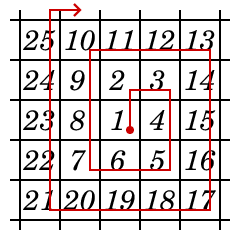
\includegraphics[scale = 0.5]{pic/105D.png}

    先将起始格子的染色器放入队首。每次把队首的染色器取出,并检查:如果这个染色器所在格子的颜色不为透明色且不为该染色器的颜色,那么按上图顺序把所有颜色为该格子颜色的格子染为该染色器的颜色。如果一个格子在染色的时候包含另一个染色器,那么把包含的这个染色器从格子中取出,并放入队尾。队列为空时结束。求共进行了多少次染色操作。

    $1 \leq n, m \leq 300$ ,颜色数不超过 $10^9$ 。
\subsubsection{算法}
\label{sec-5-4-2}

    经过分析发现,如果某次将所有颜色 $c_1$ 的格子染成了颜色 $c_2$ ,会导致两种颜色的合并,而永远不会分开。我们可以考虑维护每种颜色的格子的数目。我们还需要知道所有初始时在颜色为 $c$ 的格子上的染色器的信息。我们还需要知道,相对位置为 $(x, y)$ 的格子是第几个被访问到。每次要把颜色 $c_1$ 染成 $c_2$ 时,直接把答案加上颜色 $c_1$ 的格子数目。然后维护颜色 $c_1, c_2$ 的数目。如果第一次将 $c_1$ 染成其它颜色,我们需要按访问顺序把这些染色器加入队列。由于可以在 $O(1)$ 求出每个染色器被访问的时间,我们只需排一边序即可。

    时间复杂度 $O(nm \log nm)$ 。
\subsection{193D  Two Segments}
\label{sec-5-5}
\subsubsection{题意}
\label{sec-5-5-1}

    给定一个 $n$ 个排列 $perm$ ,一个合法区间对 $([a_1, b_1], [a_2, b_2])$ 要求满足:
\begin{enumerate}
\item $a_1 \leq b_1 < a_2 \leq b_2$
\item $perm_{a_1} \dots perm_{b_1} perm_{a_2} \dots perm_{b_2}$ 排序后任意相邻元素均差 1
\end{enumerate}

   求所有本质不同的合法区间对的数目。

   两个合法区间对本质不同,当且仅当 $\min \{perm_i \vert i \in [a_1, b_1] \cup [a_2, b_2]\}$ 不同或 $\max\{perm_i \vert i \in [a_1, b_1] \cup [a_2, b_2] \}$ 不同。

   $n \leq 3 \times 10^4$
\subsubsection{算法}
\label{sec-5-5-2}

    由于本质不同的定义,我们可以发现合法区间对事实上包含了 $[L, R]$ 内的全部的元素。

    不妨枚举 $L, R$ 。考虑如何检验是否合法。我们可以用一个 bool 数组 $t$ , $t_i$ 为真表示 $perm_i$ 在 $[L, R]$ 内。那么 $[L, R]$ 的段数就是 $t$ 中有多少段连续的 1 。如果段数不超过 2 ,那么显然可以找到一对合法区间。

    这样暴力是 $O(n^3)$ 的,远不能满足要求。我们发现,可以在枚举 $L$ 后依次枚举 $R$ ,我们可以在 $O(1)$ 的时间内维护 $t$ 有多少段。时间复杂度被优化到 $O(n^2)$ ,但仍然不能满足要求。

    再考虑依次枚举 $L$ 。枚举 $L$ 时, $t$ 的段数的变化可以用一个数组 $w$ 表示出来: $w_R$ 表示右端点枚举到 $R$ 时的段数。假设我们现在左端点枚举 $L + 1$ ,观察 $w$ 的变化。不妨令 $z$ 为 $L$ 在 $perm$ 中出现的位置,也就是 $perm_z = L$ 。
\begin{enumerate}
\item 如果 $z > 1 \and perm_{z - 1} > L$ ,可以给 $w_{perm_{z - 1} \dots n}$ 减一
\item 如果 $z < n \and perm_{z + 1} > L$ ,可以给 $w_{perm_{z + 1} \dots n}$ 减一
\item 给 $w_{L \dots n}$ 加一
\end{enumerate}

    暴力做仍然是 $O(n^2)$ 的。我们需要一个数据结构来快速支持 2 个操作:
\begin{enumerate}
\item 给一段区间全部 +/- 1
\item 查询一个后缀中 1 和 2 出现的次数
\end{enumerate}

    注意到一点, $w$ 中的任意一个元素都是正整数,那么 1 和 2 一定是最小值和次小值。用线段树维护最小值、次小值以及其出现的次数就可以了。

    时间复杂度 $O(n \log n)$ 。
\subsection{75E   Ships Shortest Path}
\label{sec-5-6}
\subsubsection{题意}
\label{sec-5-6-1}

    给定两个点 $S, T$ ,以及一个 $n$ 个点凸多边形。要从 $S$ 到 $T$ 去,路径要么在 $S$ 到 $T$ 的直线上,要么在凸多边形的边上。如果在严格多边形内部走,那么单位距离费用为 2 。否则单位距离费用为 1 。求 $S$ 到 $T$ 的最小费用。

    $2 \leq n \leq 30$ ,坐标范围不超过 100 。
\subsubsection{算法}
\label{sec-5-6-2}

    如果没有 $S$ 到 $T$ 没有交点,那么显然答案就是两点之间距离。

    如果有交点,不妨先求出交点。为了避免出现只有一个交点或者有无数个交点等特殊情况,可以把 $S$ 和 $T$ 抖动一下,使得恰好有两个交点 $x_1$ 和 $x_2$ 。我们可以构造一个图,点集为 $S, T, x_1, x_2$ 以及凸多边形的所有顶点;边集包括:
\begin{enumerate}
\item $x_1$ 和 $x_2$ 之间边。费用为两点之间的距离的两倍
\item 凸多边形内相邻两条边。费用为两点之间距离
\item $S$ 到 $x_1$ 、 $x_2$ 到 $T$ 。费用为两点之间距离。
\end{enumerate}

    对于构造出来的图求 $S$ 到 $T$ 的最短路即可。

    时间复杂度为 $O(n \log n)$ 。
\subsection{76F   Tourist}
\label{sec-5-7}
\subsubsection{题意}
\label{sec-5-7-1}

    一个无限长的数轴上,在 $t_i$ 时刻 $x_i$ 点会出现一个物品。人的移动速度为 $V$ 。求以下两种情况下人能够取的最多的物品数:
\begin{enumerate}
\item 初始时刻在 0 点
\item 初始时刻可以在任意一个点
\end{enumerate}

   $n \leq 10^5, |x_i| \leq 10^8, t_i \leq 2 \times 10^6, V \leq 1000$
\subsubsection{算法}
\label{sec-5-7-2}

    这是一个很经典的 dp 题了。我们把所有的 $t$ 乘以 $V$ ,把坐标系旋转 $45^\circ$ 后,获取物品 $i$ 后能获取物品 $j$ 的充要条件是 $x_i \leq x_j \and y_i \leq y_j$ 。

    我们把点按照 $x$ 递减, $y$ 递减的顺序排序,离散化后可以直接用线段树/树状数组维护。我用 map<int, int> 直接维护。

    如果一个点的横纵坐标都非负,那么就可以用这个点来更新第一种情况的答案。任意一个点都可以更新第二个点的答案。

    时间复杂度 $O(n \log n)$ 。
\subsection{76A   Gift}
\label{sec-5-8}
\subsubsection{题意}
\label{sec-5-8-1}

    给定一个连通无向图,每条边有两个权值 $g, s$ 。求图的一棵生成树,使得:
    $$G \max_{e \in E} g_e + S \max_{e \in E} s_e$$
    最小。

    $1 \leq n \leq 200, n - 1 \leq m \leq 50000, 1 \leq g_i, s_i, G, S \leq 10^9$
\subsubsection{算法}
\label{sec-5-8-2}

    首先可以知道,在 $\max_{e \in E} s_e$ 一定的情况下, $\max{e \in E} g_e$ 越小越好。我们不妨枚举 $\max_{e \in E} s_e$ ,然后把所有 $s_e \leq LMT$ 的边选出来,按 $g_e$ 从小到大的顺序枚举每条边。这样是可以求出 $\max_{e \in E} g_e$ 的最小值的。如果当前图连通,我们可以用当前这棵生成树来更新答案。

    但是这样复杂度是 $O(m^2 \log m)$ 的,会超。考虑优化。我们可以先把边按 $s_e$ 的大小排序,一条边一条边地加入生成树。可以知道,相邻两次枚举的生成树至多相差 2 条边:插入、删除各一条边。而树的大小是 $O(n)$ 的。我们直接维护这么一棵树,维护插入、删除一条边以及求两点之间边权最大值即可。

    另外一种处理方法为:每次把新加入的边以及上次的生成树的边归并排序,再求一棵 $g_e$ 最大值最小的生成树即可。

    时间复杂度为 $O(nm + m \log n)$ 。
\subsection{77E   Martian Food}
\label{sec-5-9}
\subsubsection{题意}
\label{sec-5-9-1}

    如图,黑色圆的半径为 $R$ ,黄色圆的半径为 $r$ ,粉色圆的半径为 $R - r$ ,且恰好与黑色圆、黄色圆相切。接下来要放置若干个绿色圆,第一个绿色圆要与黄色圆、粉色圆、黑色圆相切,第 $k > 1$ 个绿色圆要与黄色圆、黑色圆以及第 $k - 1$ 个绿色圆相切。求第 $k$ 个绿色圆的半径。
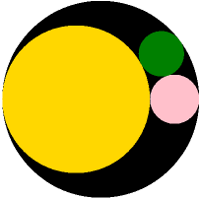
\includegraphics{pic/77E.png}
\subsubsection{算法}
\label{sec-5-9-2}

    利用 GeoGebra\footnote{http://www.geogebra.org/cms/
 } 强大的命令绘图,我画了若干个图,分析了每个圆的半径大小,并找到了规律:
    $$r_k = \frac{R}{\frac{R}{R - r} + \frac{(R - r) k^2}{r}} $$

    图像文件保留为 src/Volume-V/77E.ggb 以及 src/Volume-V/77E-2.ggb 。请用 GeoGebra 打开。

    具体证明可以利用反演。
\section{Volume VI}
\label{sec-6}
\subsection{79D   Password}
\label{sec-6-1}
\subsubsection{题意}
\label{sec-6-1-1}

    给定一个长为 $n$ 的 0/1 序列,中间有 $k$ 个位置为 1 。再给定一个长为 $l$ 的序列 $a$ ,你每次可以把连续 $a_i (1 \leq i \leq l)$ 个元素取反。求把整个序列全部变为 0 的最少步骤。

    $1 \leq n \leq 10^4, 0 \leq k \leq 10, 0 \leq l \leq 100$ 。
\subsubsection{算法}
\label{sec-6-1-2}

    由于 $n$ 这么大, $2^n$ 的状压显然不可行。

    由于涉及区间操作,我们考虑原数组 $x$ 的差分数组 $y$ : $y_i = x_i \xor x_{i - 1}$ 。易知, $y$ 中至多有 $2k$ 个 1 。而对于每次操作,我们把 $x_s, x_{s + 1}, \dots, x_{s + a_i - 1}$ 取反,在 $y$ 中对应为 $y_s, y_{s + a_i}$ 取反,也就是说每次只会改变 2 个元素。

    我们可以预处理出 $cost_{i, j}$ ,意义为把 $y_i, y_j$ 取反的最小代价。这里的 $i$ 和 $j$ 都要求 $y$ 的对应位为 1 。对于每个 $i$ ,我们可以从 $i$ 开始 BFS ,因为对一个点取反两次可以看成是不变,我们事实上在找一条路径。 由于 $y$ 中至多有 $2k$ 个位置为 1 ,BFS 一次的复杂度为 $O(nl)$ ,所以这一步的时间复杂度为 $O(nlk)$ 。

    接下来由于每次必定是消去两个 1 ,且 1 的个数不多,我们可以考虑状压 dp 。令 $f_{S}$ 表示原来的 $2k$ 个 1 中,还有 $S$ 里面的位置为 1 的最小代价。我们每次枚举编号最小的点和哪个消除即可。复杂度为 $O(k 2^{2k})$ 。

    总时间复杂度为 $O(nlk + k 2^{2k})$ 。
\subsection{81E   Pairs}
\label{sec-6-2}
\subsubsection{题意}
\label{sec-6-2-1}

    给定一个 $n$ 个点 $n$ 条边的图,每个点可能为红色或蓝色。求一个最大匹配,使得这个最大匹配在所有的最大匹配中有最多的异色匹配。要求输出方案。

    $n \leq 10^5$
\subsubsection{算法}
\label{sec-6-2-2}

    算法是很简单的。由于边数为 $n$ ,易知原图为若干棵基环外向树。先把环删掉,可以得到若干棵树。我们可以用树形 dp 得到对于每个点取不取,这棵子树内的最大匹配数,以及在最大匹配的前提下,异色匹配的最多的数目。再考虑环。对于环的部分,我们可以再写一个 dp 。由于要输出方案,转移的时候记录决策就可以了。

    当然,也可以写仙人掌 dp 。细节比较多。

    时间复杂度 $O(n)$ 。
\subsection{82E   Corridor}
\label{sec-6-3}
\subsubsection{题意}
\label{sec-6-3-1}

    如果,给定两个点 $A(0, f), B(0, -f)$ ,以及数轴上若干条不相交的线段 $(l_i, r_i)$ ,我们可以构造如下图形:

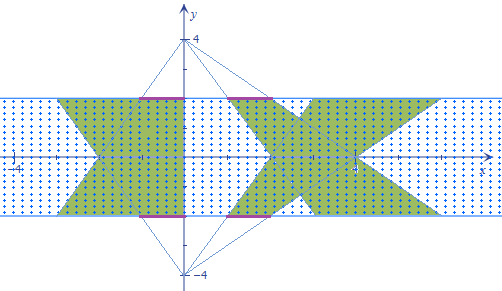
\includegraphics{pic/82E.png}

    将线段分别放在 $y = h$ 和 $y = -h$ 上, $A, B$ 分别与每条线段两端的连线所形成图形在 由 $-h \leq y \leq h$ 定义的条形区域为若干个梯形。求所有梯形的面积并。

    $n \leq 500, f \leq 10^3, h \leq 10, |l_i|, |r_i| \leq 5 \times 10^3$ 。
\subsubsection{算法}
\label{sec-6-3-2}

    最直观的想法是暴力梯形剖分。这样做的时间复杂度为 $O(n^3 \log n)$ ,会 TLE T\_{}T 。我们可以用平衡树维护,复杂度降为 $O(n^2 \log n)$ 。没写过,不知道结果。(似乎暴力维护可以过?)

    由于区间互不相交,我们可以知道每个区域至多被覆盖 2 次。把所有梯形的面积加起来,我们可以得到并的面积加上所有被覆盖 2 次的区域的面积。只要减去所有被覆盖 2 次的区域的面积即可。我们枚举两个梯形,计算其交的面积,把答案减去这么多即可。

    剩下的问题就是计算两个梯形的交。一种方法是半平面交,不容易写错。还有一种方法:所有可能出现在梯形交的点只有 12 个(斜边的交点 4 个,2 个梯形各 4 个顶点),我们依次枚举这些点,用 12 个 if 判断是否在交里面即可。

    时间复杂度 $O(n^2)$ 。
\subsection{83E   Two Subsequences}
\label{sec-6-4}
\subsubsection{题意}
\label{sec-6-4-1}

    给定一个长度为 $n$ 的字符串序列 $A$ ,每个字符串的长度均为 $l$ 。定义函数 $f(S)$ 如下:
$$
f(S) = 
\begin{cases}
$empty string$ & S = \{\} \\
s & S = \{s\}\\
$长度最小的字符串$ t $,使得$ s_1 $是$ t $的前缀,$ s_2 $是$ t $的后缀$ & S = \{s_1, s_2\} \\
f (\{f (\{s_1, s_2, \dots, s_{n - 1}\}), s_n\}) & S = \{s_1, s_2, \dots, s_n\} (n > 2) \\
\end{cases}
$$

    现要求把 $A$ 分成两个序列 $B, C$ ,使得任意两个元素的相对顺序不改变,即 $B, C$ 可以归并得到 $A$ ,且使下式最小:
    $${|f(B)| + |f (C)|}$$

    $1 \leq n \leq 2 \times 10^5, 1 \leq l \leq 20$
\subsubsection{算法}
\label{sec-6-4-2}

    我们可以设计一个 dp 。 $f_i$ 表示 $A_i$ 和 $A_{i - 1}$ 不分在同一个序列时,前 $i$ 个元素形成的 $B, C$ 的 $|f(B)| + |f(C)|$ 的最小值。转移如下:
    $$f_{i} = \min\{f_j + cost_{j - 1, c} + \sum_{k = j}^{i - 1} cost_{j, j + 1}\}$$
    其中 $cost_{a, b}$ 表示 $f(\{a, b\}) - l$ 。

    这个 dp 是 $O(n^3 l)$ 的。我们可以通过前缀和优化到 $O(n^2 l)$ ,但这样仍然不能满足要求。仔细分析发现, $cost_{j - 1, c}$ 只有 $l + 1$ 个取值。我们可以开 $t + 1$ 个数组,记录满足 $A_{j - 1}$ 最后 $x$ 位为 $y$ 的 $f_j - sum_{j}$ 的最小值,其中 $sum_j$ 为 $cost_{j, j+ 1}$ 的前缀和。每次求出一个值后 $O(t)$ 更新这个数组即可。而求出 $f$ 值也只需 $O(t)$ 扫描,时间复杂度被优化到 $O(nl)$ 。
\subsection{85E   Guard Towers}
\label{sec-6-5}
\subsubsection{题意}
\label{sec-6-5-1}

    给定平面上 $n$ 个点,要求将这 $n$ 个点染成黑白两色,使得最大的同色点的曼哈顿距离最小。求最小的值以及方案数。

    $n \leq 5000$ ,坐标范围不超过 5000 。
\subsubsection{算法}
\label{sec-6-5-2}

    这种题,一看就知道是二分答案。于是乎我写的二分答案超了。

    把所有点对之间的曼哈顿距离求出来,计数排序后从大往小扫,用并查集维护即可。

    时间复杂度 $O(n^2 \alpha(n))$ ,注意常数。
\subsection{86E   Long sequence}
\label{sec-6-6}
\subsubsection{题意}
\label{sec-6-6-1}

    对于两个长度为 $k$ 0/1 序列 $a_{1 \dots k}$ 以及 $c_{1 \dots k}$ ,我们可以生成一个无限长的 0/1 序列 $x$ :
    $$x_n = \begin{cases} a_n & n \leq k \\ \sum_{i = 1}^k c_i x_n & n > k \end{cases}$$

    我们知道 $x$ 有最小循环节。如果要求 $x$ 的循环节长度是 $2^k - 1$ ,求一组可行的 $a$ 和 $c$ 。$a$ \$c\$ 不能全为零。

    $2 \leq k \leq 50$
\subsubsection{算法}
\label{sec-6-6-2}

    首先,连续 $k$ 个 1 一定会出现,我们就不妨令 $a$ 为 $k$ 个 1 。接下来我们要求 $c$ 。

    先解决一个子问题:给定一组 $c$ ,求最小循环节是否为 $2^k - 1$ 。我们可以利用矩阵乘法,以 $k = 4$ 为例,构造如下矩阵:

$$
M = 
\left(
\begin{array}{cccc}
0 & 0 & 0 & c_4 \\
1 & 0 & 0 & c_3 \\
0 & 1 & 0 & c_2 \\
0 & 0 & 1 & c_1 \\
\end{array}
\right)
$$

    这里的矩阵乘法中的乘法为 $\and$ ,加法为 $\xor$ 。由于 $2^k - 1$ 是循环节,那么 $M^{2^k - 1}$ 必定为单位矩阵。对于 $2^k - 1$ 的所有因子 $d$ , $M^d$ 必定不为单位矩阵。我们只需枚举所有的 $\frac{2^k - 1}{p}$ 其中 $p$ 是 $2^k - 1$ 的质因子即可。由于这里矩阵乘法的特殊性,我们可以用位运算加速至 $O(k^3 \Omega(k))$ ,其中 $\Omega(k)$ 表示 $k$ 的质因子个数。

    接下来要如何求 $c$ 呢?我们只需随机即可。因为解的个数为 $O(\frac{\phi(2^k - 1)}{k})$ 的,我们期望随机次数不大,为 $O(k)$ 级。当然,打表也是可行的。

    时间复杂度为 $O(k^4)$ 。
\subsection{89D   Space mines}
\label{sec-6-7}
\subsubsection{题意}
\label{sec-6-7-1}

    三维坐标系中,给定若干个地雷一样的东西,就是一个大小为 $r_i$ 的球,从球心 $O_i$ 往不同的方向延伸出若干条线段。一个球初始位于点 $A$ ,速度向量为 $v$ ,问第一次碰到地雷是什么时候。

    $1 \leq n \leq 100$ ,每个地雷中线段的条数不超过 10 。坐标绝对值不超过 $10^5$ 。 每个球的半径不超过 100 ,每条线段的长度不超过球的半径的 1.5 倍且严格大于球的半径。每个地雷的球的半径长度不超过给定球的半径。
\subsubsection{算法}
\label{sec-6-7-2}

\begin{theorem}
  移动的球不会与给定的线段的非端点相交。
\end{theorem}
\begin{proof}
  不妨设给定的球与某个地雷有交点,如图:
\begin{center}

% \documentclass[a4paper]{article}

% \usepackage{tikz}

% \begin{document}

\begin{tikzpicture}[scale = 0.5]
  \draw[red, thick] (4, 3) circle (3cm);
  \draw[blue, thick] (0, 0) circle (2cm);
  \draw[thick] (0, 0) node[label = above: $A$] {}
           --  (4, 3) node[label = above: $O$] {};
  \draw[very thick] (-3, 0) -- (8, 0);
  % \draw (0, 2.25) -- (0, 0) node [label = below: $B$] {};
  \node[label = below: $B$] at (4, 0) {};
  \draw[thick] (4, 0) -- (4, 3);
  % \draw (6, 4   ) -- (6, 0) node [label = below: $D$] {};
\end{tikzpicture}

% \end{document}
\end{center}
  易知
\begin{equation}
  \begin{aligned}
     AB &= \sqrt{AO^2 - BO^2} \\
        &= \sqrt{(R + r)^2 - R^2} \\
        &= \sqrt{r^2 + 2Rr} \\
        &\geq \sqrt{3r^2} \\
        &> \frac{3}{2} r
  \end{aligned}
\end{equation}

\end{proof}

    所以只有可能球与球交和球与点交可能更新答案。我们可以把这两种情况统一为球与球交。利用点积可以判断出 $\vec{AO}$ 与 $v$ 是否在同一方向。利用 $A, O$ 和 $v$ 可以确定一个平面,从而可以求出 $O$ 到方向向量为 $v$ 且经过点 $A$ 的直线的距离。再利用勾股公式可以直接求出 $A$ 到交点的距离,除以 $v$ 的模即可。
\subsection{91D   Grocers Problem}
\label{sec-6-8}
\subsubsection{题意}
\label{sec-6-8-1}

    给定一个 $n$ 的排列,每次可以选择不超过 5 个位置,然后任意重排这 5 个位置的数。求最少的操作数,使得序列递增。

    $n \leq 10^5$
\subsubsection{算法}
\label{sec-6-8-2}

    这个排列由若干个环组成的。每个环是独立的,我们只需使每个环大小均为 1 即可。

    考虑一个大小不小于 4 且不为 5 的环。一次操作至多会使 4 个数到达正确的地方,于是我们可以选择任意连续 5 个元素,重排使得有 4 个位置正确。一直这样操作直到环的大小小于 4 。

    现在就只剩大小为 2 和 3 的环了。我们有 3 种方法消去环:
\begin{enumerate}
\item 同时操作两个大小分别为 2 和 3 的环
\item 同时操作两个大小为 2 的环
\item 把一个大小为 3 的环拆成两个大小为 2 的环,再分别与两个大小为 3 的环一起操作
\end{enumerate}

    可以发现,第一种操作不浪费,也就是 5 个数都到达了正确位置。第二种所有可操作的 5 个位置中浪费了 1 个,第三种所有可操作的 10 个位置中浪费了 1 个。于是可以贪心,尽量选择第一种操作,剩余的用后两种操作即可。

    时间复杂度 $O(n)$ 。
\subsection{93D   Flags}
\label{sec-6-9}
\subsubsection{题意}
\label{sec-6-9-1}

    求满足以下条件的长度介于 $L$ 到 $R$ 之间的序列个数:
\begin{enumerate}
\item 每个元素均由 1, 2, 3, 4 中的一个组成
\item 相邻两个元素不同
\item 1 和 2 不相邻
\item 3 和 4 不相邻
\item 不存在连续三个数,使得 1, 2, 3 都出现过
\item 若两序列对称后相同,则视两者为相同
\end{enumerate}

   $1 \leq L \leq R \leq 10^9$
\subsubsection{算法}
\label{sec-6-9-2}

    一眼可以看出是矩乘。长度介于 $L$ 到 $R$ 之间的序列的数目可以看成是长度不超过 $R$ 的序列个数减去长度不超过 $L - 1$ 的序列的数目。

    构造一个 26x26 的矩阵 $M$ 。由于可以从空开始,我们用 5 表示这一位没有。前 25 维表示当前序列的最后两项是什么。第 26 维用来记录答案,因为求的是长度不超过 $x$ 的序列数目。

    由于对称的只算一次,我们需要减去一部分。可以知道,长度不超过 $x$ 的自身对称的序列的个数为长度不超过 $\ceil{\frac{x}{2}}$ 的序列个数。再用矩乘求一遍即可。
\section{Volume VII}
\label{sec-7}
\subsection{97C   Winning Strategy}
\label{sec-7-1}
\subsubsection{题意}
\label{sec-7-1-1}

    给定一个长为 $n + 1$ 的序列 $p_{0 \dots n}$ ,求一无限序列 $a$ 满足
    $$\forall k, a_k \leq \sum_{i = 1}^{k - 1} (n - 2 a_i)$$
    且
    $$\Phi = \lim_{m \to \infty} \frac{\sum_{i = 1}^m p_{a_i}}{m}$$
    最大

    $n \leq 100, 0 \leq p_0 \leq p_1 \leq \dots \leq p_n \leq 1$ 
\subsubsection{算法}
\label{sec-7-1-2}

    分析第一个限制条件。易知, $a$ 后面必为循环,且 $\Phi$ 的值只和 $a$ 的循环节有关。我们只需求 $a$ 的循环节就可以了。

    令 $w_i$ 表示 $i$ 在 $a$ 的循环节中出现的频率,则 $w$ 满足
    $$\sum_{i = 0} i w_i \leq \frac{n}{2}$$
    易知,
    $$\Phi = \sum_{i = 0}^n p_i w_i$$

    在平面上构造 $n + 1$ 个点 $(i, p_i)$ ,那么 $(\sum_{i = 0} i w_i, \sum_{i = 0} p_i w_i)$ 为这 $n + 1$ 点所构成凸包内的一个点。当 $\sum_{i = 0} p_i w_i$ 取最大值时,由于 $p_i \leq p_{i + 1}$ ,所以一定这个点是凸包与 $x = \frac{n}{2}$ 的交点中 $y$ 较大的一个。

    具体实现中,由于 $n$ 比较小,我们可以 $O(n^2)$ 枚举 $x = \frac{n}{2}$ 旁的两个点,计算这条直线与 $x = \frac{n}{2}$ 的交点的纵坐标即可。

    时间复杂度 $O(n^2)$ ,可以被优化到 $O(n \log n)$ 。
\subsection{97A   Domino}
\label{sec-7-2}
\subsubsection{题意}
\label{sec-7-2-1}

    有 28 个 1x2 的多米诺骨牌,分别为 $(x, y) (0 \leq x \leq y \leq 0)$ 。如果一个包含了 28 个多米诺骨牌的图能用 14 个不相交的 2x2 的矩形覆盖,且每个矩形内的数都相同,则这个图被称为魔法图。下图为一魔法图:

\begin{center}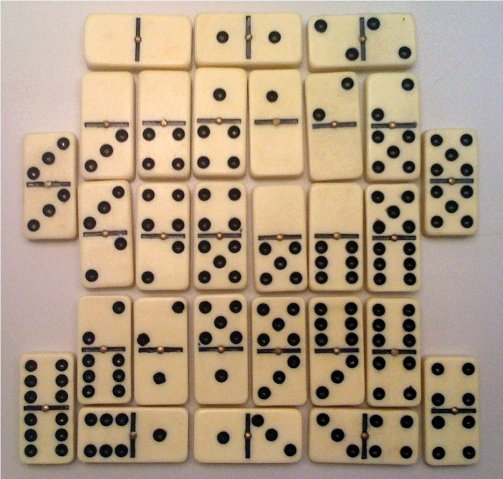
\includegraphics[scale = 0.4]{pic/97A.png}\end{center}

    给定一个 $n \times m$ 的棋盘,已用 28 个不重叠的 1x2 小片覆盖。要求用这 28 个不同的多米诺骨牌替换这 28 个小片,使得替换后这是一个魔法图。要求输出总方案数以及任意一个方案。

    $1 \leq n, m \leq 30$
\subsubsection{算法}
\label{sec-7-2-2}

    对于一组方案,我们把 0 -- 6 打乱,可以得到一个不同的合法解。所以我们只需统计有多少个本质不同的解,然后乘上 7! = 5040 即可。

    如果求本质不同的解呢?可以观察到有 7 块特殊的多米诺骨牌 $(x, x) (0 \leq x \leq 6)$ 。这种骨牌要么在一个 2x2 的矩形里,要么跨越两个矩形。我们可以快速知道有多少个第一种情况,那么第二种情况的数目就确定了。然后暴力枚举、搜索即可。
\subsection{98D   Help Monks}
\label{sec-7-3}
\subsubsection{题意}
\label{sec-7-3-1}

    现有 3 根柱子 $A, B, C$ 以及 $n$ 个盘子,盘子大小依次为 $d_i$ ,放在 $A$ 上,且大的在小的下面。现在要求将这些盘子全部移动到 $C$ 上,一次只能移动一个盘子,且任意时刻都不能有大的放在小的上方(允许相同的叠在一起),结束时要求原来在上面的盘子仍然在上面。求最少的移动次数并输出方案。

    $1 \leq n \leq 20, d_i \geq d_{i - 1}$
\subsubsection{算法}
\label{sec-7-3-2}

    令 $w_i$ 表示相对大小为 $i$ 的盘子的个数, $move-good (i, A, B, C)$ 表示将相对大小不超过 $i$ 的所有盘子从 $A$ 移到 $C$ 且顺序不变, $move-bad(i, A, B, C)$ 表示将相对大小不超过 $i$ 的盘子从 $A$ 移到 $C$ ,且除了相对大小为 $i$ 的盘子,其余的顺序不变。我们可以写出这两个函数

\begin{algorithm}
  \caption{move-good (i, A, B, C)}
  \begin{algorithmic}
    \IF{$i = 1$}
      \STATE 把前 $w_i - 1$ 个盘子从 $A$ 移到 $B$
      \STATE 把第 $w_i$ 个盘子从 $A$ 移到 $C$
      \STATE 把 $B$ 的 $w_i- 1$ 个盘子从 $B$ 移到 $C$
      \STATE exit
    \ENDIF
    \IF{$w_i = 1$}
      \STATE $move-bad (i, A, B, C)$
      \STATE exit
    \ENDIF
    \STATE $move-bad (i - 1, A, B, C)$
    \STATE 把 $A$ 的前 $w_i$ 个盘子移到 $B$
    \STATE $move-bad (i - 1, C, B, A)$
    \STATE 把 $B$ 的前 $w_i$ 个盘子移到 $C$
    \STATE $move-good (i - 1, A, B, C)$
  \end{algorithmic}
\end{algorithm}

\begin{algorithm}
  \caption{move-bad (i, A, B, C)}
  \begin{algorithmic}
    \IF{$i = 0$}
       \STATE exit
    \ENDIF
    \STATE $move-bad (i - 1, A, C, B)$
    \STATE 把 $A$ 的前 $w_i$ 个盘子移到 $B$
    \STATE $move-bad (i - 1, B, A, C)$
  \end{algorithmic}
\end{algorithm}
\subsection{98C   Help Greg the Dwarf}
\label{sec-7-4}
\subsubsection{题意}
\label{sec-7-4-1}

    如图,一个走廊一端宽 $a$ 一端宽 $b$ ,一个 $w \times l (w \leq l)$ 的矩形物体要从一端到达另一端,允许旋转。给定 $a, b, l$ 求 $w$ 的最大值。

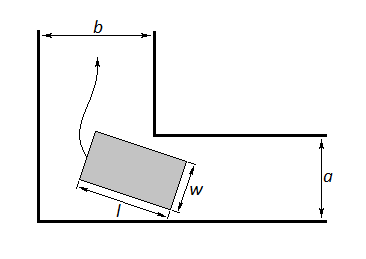
\includegraphics[scale = 0.8]{pic/98C.png}

    $a, b, l \leq 10^4$ ,要求精度 $10^{-7}$ 。
\subsubsection{算法}
\label{sec-7-4-2}

    不妨设 $a \leq b$ 。

\begin{enumerate}
\item 若 $l \leq a \leq b$ ,则答案为 $b$ 。
\item 若 $a < l \leq b$ ,则答案为 $a$ 。
\item 若 $a \leq b \leq l$ ,如图,我们有 $$w \leq f (\theta) = a \cos{\theta} + b \sin{\theta} - l \cos{\theta} \sin{\theta}$$
       所以 $w$ 为 $f(\theta)$ 的最小值。三分出 $\theta$ 即可。
\end{enumerate}
\begin{center}% \documentclass[a4paper]{article}

% \usepackage{tikz}

% \begin{document}

\begin{tikzpicture}[scale = 0.7]
  \draw [->, thick] (0, 0) -- (9, 0)
        [->, thick] (0, 0) -- (0, 7);
  \draw [blue, thick] (4, 3) -- (4, 7)
        [blue, thick] (4, 3) -- (9, 3);
  \draw (4, 3) node [above right] {$(b, a)$};
  \draw [very thick] (3, 0) arc [delta angle = -acos (0.8), start angle = 180, radius = 1cm] node [below left] {$\theta$};
  % \draw (3, 0) arc (180 :  : 1cm) -- cycle;
  \draw [red, thick, rotate around = {-acos (0.8) : (0, 3)}] (0, 3) rectangle (5, 5.4);
\end{tikzpicture}

% \end{document}
\end{center}
\subsection{191D  Metro Scheme}
\label{sec-7-5}
\subsubsection{题意}
\label{sec-7-5-1}

    给定一个无向图,保证每个点至多出现在一个简单环上。每次可以覆盖一条路径或一个简单环,求最小覆盖。

    $n \leq 10^5, m \leq 3 \times 10^5$
\subsubsection{算法}
\label{sec-7-5-2}

    由于图的特殊性质,对于一个环,如果这个环上有至少两个点连接出去,那么这个环上的所有边就可以在覆盖这些点的时候顺便覆盖掉。如果环上只有一个点连接出去,那么就用一次覆盖,把这个环覆盖掉。

    剩下的就是若干棵树,我们要用最少的路径把这些树的边全部覆盖。这是一个经典的 dp 问题。不过我们也可以用贪心来解决。在此不在赘述。

    时间复杂度 $O(n +m)$ 。
\subsection{164D  Minimum Diameter}
\label{sec-7-6}
\subsubsection{题意}
\label{sec-7-6-1}

    给定平面上 $n$ 个点,要求删掉恰好 $k$ 个点,使得剩下的大小为 $n - k$ 的点集的直径尽量小。一个点集的直径指点集中两点之间距离的最大值。

    $n \leq 1000, k \leq 30$ ,坐标范围为 32000 。
\subsubsection{算法}
\label{sec-7-6-2}

    由于要使最大值最小,我们可以考虑二分答案。二分答案后,有些点不能被同时选中。我们用一个图来表示这个关系,顶点表示点,边表示关系。那么当前答案是否合法等价于这个图的最小覆盖集的大小是否不超过 $k$ 。由于求最小覆盖集的大小是 NPC 的,而且这里 $k$ 不大,我们可以考虑关于 $k$ 的指数级算法。

\begin{theorem}
  \label{thr:164D}
  在搜索过程中,如果当前连通块的大小大于 2 ,那么选择一个度数不小于 2 的点加入覆盖集中,一定可以得到一个最优解。
\end{theorem}

    从 \ref{thr:164D} 我们可以确定一个搜索算法:对于一个度数不小于 2 的点,我们枚举它是否在覆盖集中,如果它在,那么覆盖集中剩下点的数目会减少一。否则,它的邻居必须全部在覆盖集中,由于度数不小于 2 ,那么至少有 2 个点加入覆盖集,覆盖集剩下点的数目至少减少 2 。那么每次搜索的时间复杂度为 $f(K) \leq f(K - 1) + f(K - 2)$ 。可以得到 $f(K) \leq fib_K$ ,其中 $fib_K$ 表示第 $K$ 个 Fibonacci 数。而 $fib_{30} = 832040$ 在可承受范围内。

    时间复杂度为 $O(\log n K fib_K)$ 。
\subsection{150E  Freezing with Style}
\label{sec-7-7}
\subsubsection{题意}
\label{sec-7-7-1}

    给定一棵大小为 $n$ 的树,求一条路径,长度在 $[L, R]$ 内,且组成这条路径的边的中位数最大。一个长度为 $n$ 的序列 $x_{1 \dots n}$ 的中位数为将 $x$ 升序排序后的 $x_{\ceil{\frac{n}{2}}}$ 。输出方案。

    $1 \leq L \leq R < n \leq 10^5$ ,边权范围不超过 $10^9$ 。
\subsubsection{算法}
\label{sec-7-7-2}

    由于是一条全局的路径,我们可以考虑使用树上的分治算法\footnote{参考 2009 年集训队论文,漆子超《分治算法在树的路径问题中的应用》
 }。在这个题中,我使用的是点分治。

    中位数不好处理,我们可以二分答案,并对图做相应的修改:边的权如果不小于二分的答案 $ans$ ,则边权为 1 否则边权为 -1 。这样修改后,我们的目的是找到一条长度在 $[L, R]$ 内的权值大于 0 的路径。每次 $O(n)$ 求出树的重心 $v$ ,$v$ 把树剖成若干棵子树。我们处理过 $v$ 的所有路径,然后递归处理每棵子树。显然,对于一棵子树 $x$ ,我们只需知道 $v$ 到所有深度为 $d$ 的点的最大权路径即可。为了易于处理,我们把每棵子树按高度从小到大排序,每次加入一棵子树,并求出这棵子树和所有已经处理过的子树的答案。我们可以使用单调队列来处理。处理一棵子树的复杂度为 $O(height_x)$ 的,所以处理所有过点 $v$ 的路径的复杂度为 $O(size_v)$ 。由于点分治还带有一个 $\log$ ,所以整体时间复杂度为 $O(n \log^2 n)$ 。
\subsection{101E  Candies and Stones}
\label{sec-7-8}
\subsubsection{题意}
\label{sec-7-8-1}

    有两个数 $a, b$ ,一开始都为 0 。每次可以把 $a, b$ 中的一个数增加 1 ,得到 $(x_a + y_b) \% p$ 的分数。要求任意时刻 $a < n, b < m$ 。求当 $a = n - 1, b = m - 1$ 时分数总和的最大值。要求输出方案。时限 15s ,空限 45M 。

    $1 \leq n, m \leq 20000, x, y \leq 20000, p \leq 10^9$
\subsubsection{算法}
\label{sec-7-8-2}

    首先我们可以设计一个 $O(nm)$ 的 dp :令 $f_{i, j}$ 表示 $a = i, b= j$ 时的最大总分数,每次转移时枚举是给 $a$ 加还是给 $b$ 加即可。

    但是这个 dp 有个问题,就是空间要求太大。我们可以用滚动数组来优化。但是这样无法记录方案了。我们可以考虑用分治来优化。令 $solve(x_1, y_1, x_2, y_2)$ 表示求从 $(a, b) = (x_1, y_1)$ 转移至 $(a, b) = (x_2, y_2)$ 的方案。我们可以用 $O((x_2 - x_1)(y_2 - y_1))$ 的时间求出 $(x_1, y_1)$ 转移至 $(mid, y)$ 时的最优解,以及 $(mid, y)$ 转移至 $(x_2, y_2)$ 时的最优解,其中 $mid = \floor{\frac{x_1 + x_2}{2}}$ ,然后枚举 $y$ ,找到最优的 $y$ ,递归调用 $solve(x_1, y_1, mid, y)$ 以及 $solve(mid + 1, y, x_2, y_2)$ 即可。时间复杂度为:
    $$g(x_1, y_1, x_2, y_2) = g(x_1, y_1, mid, y) + g(mid + 1, y, x_2, y_2) + O(nm) = O(nm)$$

    时间复杂度为 $O(nm)$ ,由于每次递归的时候重新求一部分 $f$ ,可以直接用滚动数组,所以空间复杂度为 $O(m)$ 。
\subsection{103E  Buying Sets}
\label{sec-7-9}
\subsubsection{题意}
\label{sec-7-9-1}

    给定 $n$ 个集合,且每个集合有一个权。这 $n$ 个集合的任意 $p$ 个集合的并的大小总是不小于 $p$ 。请选出一个数 $k$ ,然后选 $k$ 个集合,使得这 $k$ 个集合的并的大小恰好为 $k$ ,且这 $k$ 个集合的权之和最小。 $k$ 允许为 0 。

    $n \leq 300, |S| \leq n$ ,每个集合的权不超过 $10^6$ 。
\subsubsection{算法}
\label{sec-7-9-2}

    我们把原问题分解为两个子问题:
\begin{enumerate}
\item 找 $k$ 个集合,使得这 $k$ 个集合的并的大小恰好为 $k$
\item 找一个权最小的满足上述条件的 $k$ 个集合
\end{enumerate}

    我们可以发现这两个问题都可以用网络流来做。第一个问题可以看成是求 $|S| - |\cup S|$ 的最小值,我们令选取一个集合有 1 的收益,选取 1 个元素有 -1 的收益,选取一个集合就必须选取集合内所有元素,由题意知总收益不会大于 0 ,我们的目标是令总收益为 0 ,最大化总收益即可这是经典的最大权闭合图模型。对于第二个问题,我们可以直接在第一个问题的基础上做,我们把权变为两个关键字,选取一个集合的收益为 $(1, w_i)$ ,其中 $w_i$ 表示这个集合的权,选取一个元素的收益为 $(-1, 0)$ ,我们要在令第一关键字最大的前提下,令第二关键字最小。直接令收益为,第一关键字乘上一个足够大的数,加上第二关键字即可。

    当然用 Hall's 定理也是可以做的。

    时间复杂度 $O(maxflow (2n + 2, \sum |S| + 2n))$ 。
\section{Volume VIII}
\label{sec-8}
\subsection{105E  Lift and Throw}
\label{sec-8-1}
\subsubsection{题意}
\label{sec-8-1-1}

    射线 $y = 0 (x > 0)$ 上有 3 个人,每个人都在一个整点上。每个人有两个参数 movement range $R_m$ 以及 throwing range $R_t$ 。每个人可以执行以下操作,且每个操作至多执行一次:
\begin{enumerate}
\item 左右移动到距离为 $x \leq R_m$ 的点,要求目标点上没人,且此人未被举起
\item 若 $a$ 与 $b$ 距离为 1 , 且 $b$ 尚未被举起,则 $a$ 可将 $b$ 举起, $b$ 移动到 $a$ 的位置
\item 若 $a$ 将 $b$ 举起,则 $a$ 可将 $b$ 扔到距离不超过 $x \leq R_t$ 的点,要求目标点上没人
\item 被举起的人不能进行任何操作,允许 $a$ 举起 $b$ ,$b$ 举起 $c$
\end{enumerate}
    求坐标最大的人的坐标最大是多少。

    保证每个人的初始位置、 $R_m, R_t$ 均不超过 10 。
\subsubsection{算法}
\label{sec-8-1-2}

    搜索即可。我的暴搜过不了,于是加了个最优性剪枝:
\begin{improve}
   令三人最大的坐标为 $k$ ,然后枚举其余的人,如果还没有扔,就把 $k$ 加上 $R_t$ ,如果还没有移动,那就把 $k$ 加上 $R_t$ 。如果在这之后 $k$ 仍然小于已有的最优解,那么肯定这棵搜索子树内搜不到更优的解了,直接剪掉。
\end{improve}

    时间复杂度 $O(40^9)$ 。
\subsection{107D  Crime Management}
\label{sec-8-2}
\subsubsection{题意}
\label{sec-8-2-1}

    已知一个字符串长度为 $n$ ,且对于每个字符 $c$ ,均存在 $m \in S_c$ ,意义为字符 $c$ 出现的次数至少是某个 $m$ 的倍数。若对于字符 $c$ 没有条件,则 $c$ 不允许出现。求所有满足要求的字符串的个数。

    $n \leq 10^18, \Pi_c \Pi_{m \in S_c} m \leq 123$
\subsubsection{算法}
\label{sec-8-2-2}

    对于一个字符 $c$ ,我们只需储存其出现次数模 $\Pi_{m \in S_c} m$ 即可,由于 $\Pi_c \Pi_{m \in S_c} \leq 123$ ,我们可以用一个 123 以内的数把所有字符出现的次数模 $\Pi_{m \in S_c} m$ 记录下来。令 $f_{i, x}$ 表示长度为 $i$ 的串,模的信息为 $x$ 的方案数。转移时枚举下一个字符即可。最后答案即为 $\sum_{x \text{is valid}} f_{n, x}$ ,要求 $x$ 合法,即每个字符 $c$ 出现的次数至少是某个 $m$ 的倍数。

    由于 $f$ 的转移是线性递推,我们可以用矩阵乘法加速。

    时间复杂度为 $O((\Pi_c \Pi_{m \in S_c})^3 \log n)$ 。
\subsection{113D  Museum}
\label{sec-8-3}
\subsubsection{题意}
\label{sec-8-3-1}

    给定一个连通无向图 $G = (|V| = n, |E| = m)$ ,有两个人在点 $a$ 与点 $b$ 。每个人的移动规则如下:若两人在同一个点,则不移动;否则假设在点 $v$ ,则有 $p_v$ 的概率留在原地,否则有 $1 - p_v$ 的概率随机选择一条边走。无限步后,两人同一个点的概率为 1 。求最后两人同时停在每个点的概率。

    $n \leq 22, 0.01 \leq p_i \leq 0.99$
\subsubsection{算法}
\label{sec-8-3-2}

    令 $f_{a, b}$ 表示两人初始一人在 $a$ ,另一人在 $b$ ,两人同时停在 $v$ 的概率。我们有:
    $$f_{a, b} = \sum_{(x, y)} prob_{(a, b) \to (x, y)} f_{x, y}$$
    当枚举最后同时停在点 $v$ 时,我们令 $f_{i,i} = [i = v]$ 。

    这样,我们就有 ${n \choose 2}$ 个方程以及 ${n \choose 2}$ 个未知数,可以用高斯消元在 $O(n^6)$ 的时间内求出最后同时停在点 $v$ 的概率。枚举 $v$ ,时间复杂度变为 $O(n^7)$ ,承受不了,还要优化。我们用矩阵把方程组写成 $Ax = B$ 的形式。可以发现,枚举 $v$ 时, $A$ 总是不变的。也就是说每次消元的过程是不变的,我们可以只进行一次消元,顺便求出所有的 $x$ 。

    时间复杂度为 $O(n^6)$ ,常数较小。
\subsection{115D  Unambiguous Arithmetic Expression}
\label{sec-8-4}
\subsubsection{题意}
\label{sec-8-4-1}

\begin{definition}
  定义 UAE(\textit{unambiguous arithmetic expression}) 为:
  \begin{itemize}
  \item 所有的非负整数都是 UAE ,允许前导零
  \item 如果 $X, Y$ 是 UAE ,那么 $(X)+(Y), (X)-(Y), (X)*(Y), (X)/(Y)$ 都是 UAE
  \item 如果 $X$ 是 UAE ,那么 $-(X), +(X)$ 都是 UAE
  \end{itemize}
\end{definition}

    给定一个字符串 $S$ ,求有多少个 UAE 把括号去掉后和 $S$ 相等。

    $|S| \leq 2000$
\subsubsection{算法}
\label{sec-8-4-2}

    首先我们对 $S$ 进行处理。可以发现, * 和 / 是等价的, + 和 - 是等价的。先把无解的情况特判掉。如果最后一个字符是一个运算符,那么显然无解。如果两个 * 连在一起,也无解,否则一定有解。

    分析 $+(X)$ 这种情况。可以知道, + 之前必定为一运算符,我们可以在 + 之前再加入一个数字,使其变成 $(0)+(X)$ 这样的串。那么现在,我们把原题以另一种方法叙述出来:

\begin{problem}
  给定一个长为 $n$ 的序列,每次可以合并两个相邻元素,且某些元素在第一次合并的时候必须是前面的那个元素,即只能和他后面的合并。求最后合并成一个的方案数。

  两个方案不同,当且仅当存在一个合并后的元素只在某一个方案中出现。
\end{problem}

    这个问题我们可以用 dp 来解决。令 $f_{i, j}$ 表示前 $i$ 个元素经过一系列合并后,还剩下 $j$ 个元素的方案数。转移为:
    $$f_{i, j} = \begin{cases} f_{i - 1, j - 1} & \text{第 $i$ 个元素合并时有限制} \\ \sum_{k = j - 1}^i f_{i - 1, k} & \text{otherwise} \\ \end{cases}$$ 。

    第二种转移可以用前缀和优化: $$f_{i, j} = f_{i - 1, j - 1} + f_{i, j + 1}$$
    所以转移可以被优化到 $O(1)$ 

    时间复杂度为 $O(n^2)$ 。
\subsection{120I  Luck is in Numbers}
\label{sec-8-5}
\subsubsection{题意}
\label{sec-8-5-1}

    如图,所有的数字均用 7 根线段表示。定义一个长为 $2n$ 的数字串的权为:所有既在第 $i (1 \leq i \leq n)$ 个数字,又在第 $i +n$ 个数字中出现的线段的数目。

    给定长为 $2n$ 的数字串,求一个同长、权严格比给定串的权大、字典序严格比给定串大且字典序最小的数字串。

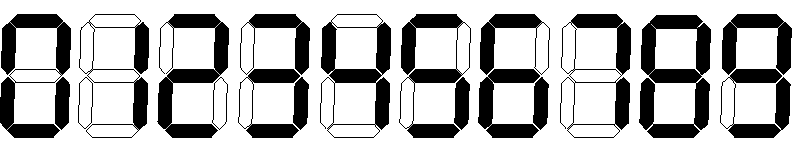
\includegraphics[scale = 0.6]{pic/120I.png}

    $n \leq 10^5$
\subsubsection{算法}
\label{sec-8-5-2}

    贪心即可。

    我们预处理出两个数组 $opt$ 和 $pre$ ,分别表示前 $i$ 个字符包含的线段的个数,以及同时出现在前 $i$ 个字符和中间 $[n + 1, n + i]$ 这个区间内的线段个数。从前往后扫描每个字符,如果把某个字符替换成另一个字符 $x$ 后,这个字符串的最大的可能的权可以通过 $pre$ 和 $opt$ 两个数组得到。如果可以增加权,那么就可以 break 了。

    如何构造方案?从 break 的地方开始,从前往后依次枚举每个位置的字符,利用 $pre$ 和 $opt$ 我们可以知道如果一个位置填上某个字符,那么这个字符串的最大的权是多少。

    时间复杂度 $O(n)$ ,注意公式不要错即可。
\subsection{123E  Maze}
\label{sec-8-6}
\subsubsection{题意}
\label{sec-8-6-1}

    给定一棵树,描述 dfs 过程如下:
\begin{algorithm}
  \label{algo:123E-dfs}
  \caption{dfs (x)}
  \begin{algorithmic}
    \IF{$x$ 为出口}
      \STATE 完成 dfs 
    \ENDIF
    \STATE flag[x] $\leftarrow$ TRUE
    \STATE 随机打乱 $x$ 的所有相邻的点 $V(x)$
    \FOR {$i = 1$ to $|V (x)|$}
      \IF {flag[V[i]] = FALSE}
         \STATE count $\leftarrow$ count + 1
         \STATE dfs (V[i])
      \ENDIF
    \ENDFOR
    \STATE count $\leftarrow$ count + 1
  \end{algorithmic}
\end{algorithm}
    现在每个点有两个值 $x_i$ 和 $y_i$ ,分别表示这个点成为起点的可能性为 $\frac{x_i}{\sum x_i}$ 和 $\frac{y_i}{\sum y_i}$ 。求 $dfs (x)$ 后, count 的期望大小。

    $n \leq 10^5, x_i, y_i \leq 10^3$
\subsubsection{算法}
\label{sec-8-6-2}

    考虑化简 $u$ 为起点, $v$ 为终点时, count 的期望大小。不妨另 $v$ 为根,那么如果 $x$ 不在 $u-v$ 路径上,那么肯定找不到 $v$ ,所以 count 的值为 $2 size_x$ 。而如果 $x$ 在 $u-v$ 路径上,那么对于 $x$ 的未访问邻居 $w$ ,均有 0.5 的可能性在访问 $v$ 之前访问到 $w$ ,所以每棵子树对答案的贡献为子树大小。所以最后答案为:以 $v$ 为根, $u-v$ 最后一个点所代表的子树的大小。

    我们考虑每个点作为终点的情况。我们在 dfs 的时候可以顺便维护子树大小以及子树中 $x_i$ 的和,那么我们可以知道起点在任意一个子树中的概率,以及在这棵子树时的期望答案。把每个点对答案的贡献累加即可。
\subsection{125E  MST Company}
\label{sec-8-7}
\subsubsection{题意}
\label{sec-8-7-1}

    给定一个图,求点 1 的度数恰好为 $k$ 的生成树的最小权值。要求输出方案。

    $n \leq 5000, m \leq 10^5, 0 \leq k \leq n$
\subsubsection{算法}
\label{sec-8-7-2}

    如果我们把每条和 1 有关的边权全部减去 $v$ ,求最小生成树,那么 MST 中和 1 有关的边的数量随着 $v$ 的增大而非降。二分 $v$ ,每次尽量选择和 1 有关的边,可以求出当 $v$ 至少为 $x$ 时, MST 中有不小于 $k$ 条和 1 有关的边。

    接下来考虑如何求方案。我们先求把每条边的权减去 $x - 1$ 后的 MST ,可以知道这时候点 1 的度数一定小于 $k$ ,且当 $v = x$ 时,这些边仍然是要选的。然后再求把每条边的权减去 $x$ 后的 MST 。考虑为啥 $x - 1$ 不行而 $x$ 可以,因为存在和 1 有关的边使得减去 $x$ 后在尽量选择和 1 有关的边这个前提下被选择。而这些边都是可以被和 1 无关的边替代的,我们在中间任选若干条,使 1 的度数等于 $k$ 即可。这样和 1 有关的边就确定了。其余的边可以直接求 MST 得到。

    具体细节可以参考去年陈立杰的集训队互测试题《tree》。
\subsection{193E  Fibonacci Number}
\label{sec-8-8}
\subsubsection{题意}
\label{sec-8-8-1}

    给定一个非负整数 $x$ ,求最小的 $t$ 使得 $fib_t \equiv x \pmod{10^{13}}$ 。

    $0 \leq x < 10^{13}$
\subsubsection{算法}
\label{sec-8-8-2}

    通过打表可以发现, $\{fib_i \mod{5^{t}}\}$ 的周期是 $5^{t} \times 4$ , $\{fib_i \mod{2^t}\}$ 的周期是 $2^{t - 1} \times 3$ 。我们可以分两部分处理,求出一个循环节内所有 $fib_i \equiv x \pmod{5^{13}}$ 的 $i$ ,以及 $fib_i \equiv x \pmod{2^{13}}$ 的 $i$ ,然后再用中国剩余定理就可以求出 $t$ 了。

    对于 $fib_i \equiv x \pmod{2^{13}}$ 的 $i$ ,由于循环节较短,可以直接求。

    对于 $fib_i \equiv x \pmod{5^{13}}$ 的 $i$ ,循环节长达 $5 \times 10^{9}$ 级,不能直接求。我们可以考虑一边枚举一边求。如果 $fib_i \equiv x \pmod{5^{13}}$ ,则一定有 $fib_i \equiv x \pmod{5^{9}}$ 。而 $\{fib_i \mod{5^9}\}$ 的循环节长度只有 $8 \times 10^6$ ,可以直接求。求得了满足 $fib_i \equiv x \pmod{5^9}$ 的 $i$ 后,我们枚举循环节内所有和 $i$ 关于 $5^9$ 同余的数 $j$ ,求出 $fib_j \mod{5^{13}}$ 即可。

    时间复杂度为 $O(1)$ ,常数为 $O(2 \times 5^{4} \log 10^{13} + 5^9 + 2^{12} \times 3)$ 。
\subsection{145D  Lucky Pair}
\label{sec-8-9}
\subsubsection{题意}
\label{sec-8-9-1}

    一个数字被称为幸运的,当且仅当它的每一位要么是 4 要么是 7 。

    给定一个长为 $n$ 的序列,求有多少个区间对 $[L_1, R_1], [L_2, R_2]$ ,使得 $L_1 \leq R_1 < L_2 \leq R_2$ ,且不存在一个幸运数字同时在 $[L_1, R_1]$ 和 $[L_2, R_2]$ 中出现。

    $n \leq 10^5$ ,且幸运数字出现次数不超过 1000 。
\subsubsection{算法}
\label{sec-8-9-2}

    我们把所有区间对分成两种,按照第一个区间中是否包括幸运数字。

\begin{enumerate}
\item 如果第一个区间中不包括幸运数字,那么我们可以枚举 $R_1$ ,找到在这之前最近的幸运数字,可以知道有多少个 $L_1$ 满足要求。由于 $[L_1, R_1]$ 中不包括幸运数字,那么 $[L_2, R_2]$ 是没有限制的。这可以通过组合数算出来。
\item 如果第一个区间中不包括幸运数字,我们枚举这个区间中第一个出现的幸运数字,然后从后往前枚举最后一个幸运数字的位置。我们发现,已经在 $[L_1, R_1]$ 中出现的幸运数字是不能在 $[L_2, R_2]$ 中出现的,所以有若干个数字是不能选的。也就是有若干个障碍点。障碍点把 $[R_2 + 1, n]$ 分成若干个区间,而 $[L_2, R_2]$ 必定是某个区间的子区间。还可以发现,每次改变最后一个幸运数字的位置时,会有若干次相邻区间合并。我们用数据结构维护区间就可以了。
\end{enumerate}

   时间复杂度 $O(m^2 \log m + n)$ ,其中 $m$ 为幸运数字出现次数。
\section{Volume IX}
\label{sec-9}
\subsection{132E  Bits of merry old England}
\label{sec-9-1}
\subsubsection{题意}
\label{sec-9-1-1}

    给定一个长为 $n$ 的序列,现在一个打字机有 $m$ 个缓冲槽,有两个操作:
\begin{enumerate}
\item 将某个缓冲槽内的数置为 $x$ ,代价为 $x$ 的二进制表示中, 1 的个数
\item 将某个缓冲槽内的数打印出来,无代价
\end{enumerate}
   现在要求将这个序列依次输出,求最小代价,并输出方案。
\subsubsection{算法}
\label{sec-9-1-2}

    网络流。

    我们把每个元素看成是一个节点,一条增广路看成是一个缓冲槽中的数字的变化情况。新建 $n + 1$ 个辅助节点 $aux_{0 \dots n}$ 。每个辅助节点表示可以用的缓冲槽的集合。可以构造如下图:
\begin{enumerate}
\item $\forall 1 \leq i \leq n$ ,加入一条 $aux_{i - 1}$ 到 $i$ 的边,流量限制为 1 ,费用为把第 $i$ 个数输入某个缓冲槽的代价。这种边的意义是将某个缓冲槽内的数替换为第 $i$ 个数。
\item $\forall 1 \leq i \leq n$ ,加入一条 $aux_{i - 1}$ 到 $aux_i$ 的边,流量限制为 $m$ ,费用为 0 ,意义为上次没用完的缓冲槽这次可以接着用。
\item $\forall 1 \leq i \leq n$ ,加入一条 $i$ 到 $aux_i$ 的边,流量限制为 1 ,费用为 0 ,意义为这个缓冲槽用完了,值会改变,进行回收。
\item 如果第 $i$ 个元素和第 $j > i$ 个元素是一样的,加入一条 $i$ 到 $j$ 的边,流量为 1 ,费用为 0 ,表示这个缓冲槽输出 $i$ 后接着输出 $j$ 。
\end{enumerate}

    如果限制代表每个元素的节点必须走到,那么这个图的流量不超过 $m$ 的最小费用可行流就是答案。这样对于每个点有个下界,我们用拆点的技巧即可。

    至于方案的输出,观察每条边有没有流量即可。

    复杂度 $O(MincostMaxflow (3n + 2, 6m))$
\subsection{138D  World of Darkraft}
\label{sec-9-2}
\subsubsection{题意}
\label{sec-9-2-1}

    给定一个 $n \times m$ 的矩形,每个元素为 \texttt{LRX} 中的一个,初始时每个元素都是活跃的。两个人博弈,每次选择一个活跃元素,然后将一些元素设为不活跃:
\begin{enumerate}
\item 如果这个元素是 \texttt{L} ,不活跃节点为这个元素的左下至右上这条线上的若干个点
\item 如果这个元素是 \texttt{R} ,不活跃节点为这个元素的右下至左上这条线上的若干个点
\item 如果这个元素是 \texttt{X} ,不活跃节点为经过这个元素的两条对角线上的若干个点
\end{enumerate}
    注意,每次修改时均为从这个点开始,向每条线的两端移动。如果当前格子已被设为不活跃节点,那么就停止这个方向的操作。

    问先手必胜还是后手必胜。

    $n, m \leq 20$
\subsubsection{算法}
\label{sec-9-2-2}

    我们发现,任意时刻的总局面总是由若干个部分游戏组成,这让我们想到了 SG 函数。经过分析可以得到:
\begin{theorem}
  \begin{itemize}
  \item 原游戏可以分解为两个游戏:黑白染色后黑色的为一个游戏,白色的为一个游戏
  \item 任意一个子游戏均为原矩形与一矩形的交
  \end{itemize}
\end{theorem}

    这样,我们可以考虑用 $f_{ls, rs, ld, rd}$ 来表示一个子游戏的 SG 值,这个子游戏为 $ls \leq x + y \leq rs, rd \leq x - y \leq rd$  这个矩形与原矩形的交。枚举这个所有可能的点即可。

    时间复杂度 $O(n^6)$ 。
\subsection{140F  New Year Snowflake}
\label{sec-9-3}
\subsubsection{题意}
\label{sec-9-3-1}

    给定一个大小为 $n$ 的点集,你可以添加不超过 $k$ 个点,使得存在一个点 $p$ ,对于点集内任意一点 $q$ 均存在 $q$ 关于 $p$ 的对称点。要求输出所有不同的 $p$ 。

    $n \leq 2 \times 10^5, 0 \leq k \leq 10$
\subsubsection{算法}
\label{sec-9-3-2}

    我们现将点集内的点排序, $x$ 为第一关键字, $y$ 为第二关键字。

    我们枚举最前面有 $L$ 个点不能匹配,最后面有 $R$ 个点不能匹配,那么对称中心一定是第 $L + 1$ 个点与第 $n - R$ 个点的中点。然后 $O(n)$ 扫一遍,可以知道有内部有多少个点不能匹配。如果不超过 $k$ ,则可以加入答案。

    易知 $L + R \leq k$ ,所以时间复杂度 $O(n k^2)$ 
\subsection{147B  Smile House}
\label{sec-9-4}
\subsubsection{题意}
\label{sec-9-4-1}

    给定一个无重边无自环的边权无向图,求一个最小的 \$k4 ,使得一个大小为 $k$ 的环的长度为正。

    $n \leq 300, n - 1 \leq m \leq {n \choose 2}$ ,边权绝对值不超过 $10^4$ 。
\subsubsection{算法}
\label{sec-9-4-2}

    我们用邻接矩阵来表示这个图。这里重新定义矩阵乘法:矩阵 $A$ 乘上矩阵 $B$ 得到的矩阵 $C$ 为:
    $$C_{i, j} = \max_{1 \leq k \leq n} \{A_{i, j}, B_{i, j}, A_{i, k} + B_{k, j}\}$$

    这个特殊的矩阵乘法的意义为,若 $A$ 表示经过不超过 $a$ 条边的两点间路径的最大值, $B_{i, j}$ 表示经过不超过 $b$ 条边的两点间路径的最大值,那么 $C$ 表示经过不超过 $a + b$ 条边的两点间路径的最大值。这样,我们可以在 $O(n^3 \log n)$ 的时间内用倍增求出任意两点间不超过 $2^k$ 条边的路径的最大值。接下来,我们可以利用倍增的数组进行二分,可以在 $O(n^3 \log n)$ 的时间内求出答案。

    时间复杂度 $O(n^3 \log n)$ 。
\subsection{152D  Frames}
\label{sec-9-5}
\subsubsection{题意}
\label{sec-9-5-1}

    给定一个 $n \times m$ 的字符数组,要求两个边界平行于坐标轴的矩形,使得这两个矩形的边界恰好能覆盖所有的 \texttt{\#} ,且任意一个矩形的任意一条边的长度不小于 3 。

    $n, m \leq 10^3$
\subsubsection{算法}
\label{sec-9-5-2}

    由于只有两个矩形,我们可以考虑暴力枚举。我们求出所有的行、列,使得这一行/列中包括至少 3 个连续 \texttt{\#} 。考虑如下情况:
\begin{verbatim}
..........
.....####.
.....####.
.....####.
.....####.
.....####.
.....####.
.....####.
.....####.
..........
..........
\end{verbatim}

    这个图的确可以找出两个矩形,但是存在很多行有连续 3 个 \texttt{\#} 。可以注意到:所有 $x, y$ 只有最小的两个和最大的两个是有用的。我们只需保存这两个即可。除去其余的后,我们只有至多 4 个不同的 $x$ 和 4 个不同的 $y$ ,暴力枚举即可。每次枚举两个矩形的边界后,枚举每个 \texttt{\#} 判断是否在边界上,顺便记录每个矩形的边界上已经出现了多少个 \texttt{\#} ,这样可以比较轻松地判断出是否覆盖了非 \texttt{\#} 的点。

    时间复杂度 $O(nm)$ 。
\subsection{183D  T-shirt}
\label{sec-9-6}
\subsubsection{题意}
\label{sec-9-6-1}

    有 $n$ 个人以及 $m$ 种衣服,其中第 $i$ 个人合适的衣服为第 $j$ 种衣服的概率为 $p_{i, j}$ ,现在可以带 $n$ 件衣服,使得期望拿到合适衣服的人数最多。

    $n \leq 3000, m \leq 300$
\subsubsection{算法}
\label{sec-9-6-2}

    令 $w_{x, y}$ 表示对于第 $x$ 种衣服,恰好有 $y$ 个人合适的衣服为 $x$ 的概率;令 $E_{x, y}$ 表示对于第 $x$ 种衣服,带 $y$ 件去期望拿到合适衣服的人的个数。可得:
    $$E_{x, y} = \sum_{t = 0}^{n} w_{x, t} \min (y, t)$$

    如果暴力求出 $w$ 那么复杂度将会是 $O(n^2m)$ ,需要优化。易知 $E_{x, 0} = 0$ 。注意到:
\[
\begin{array}{rcl}
E_{x, y + 1} - E_{x, y} & = & \sum_{t = 0}^n w_{x, t} \min (y + 1, t) - \sum_{t = 0}^n w_{x, t} \min (y, t) \\
 & = & \sum_{t = y + 1}^n w_{x, t} \\
 & = & 1 - \sum_{t = 0}^y w_{x, t} \\
\end{array}
\]

     可得 $E_{x, y + 2} - E_{x, y + 1} \leq E_{x, y + 1} - E_{x, y}$ 。于是我们可以设计一个贪心算法:不妨令 $N_x$ 表示最优方案中第 $x$ 种衣服的数目。初始时令 $N_x = 0$ 。我们每一次找一个使得最大的 $E_{x, N_x + 1} - E_{x, N_x}$ 的 $x$ 并令 $N_x$ 增加 1 。可以证明,这样做一定可以得到最优方案。

     可是我们还是要求 $w$ 。但是,观察所需求的 $w$ 可得, 需要求的 $w$ 是连续的,也就是对于相同的 $x$ ,所有要求 $w_{x, y}$ 的 $y$ 是连续的。这个性质保证我们至多遍历 $O(n^2)$ 个值,每次转移是 $O(1)$ 的。所以花在 $w$ 上的时间复杂度为 $O(n^2)$ 。

     总体时间复杂度为 $O(n(n+m))$ 。
\subsection{217E  Alien DNA}
\label{sec-9-7}
\subsubsection{题意}
\label{sec-9-7-1}

\begin{definition}
  一个串 $S_{1 \dots n}$ 的变异串为: $S_2 S_4 \dots S_{2 \floor{\frac{n}{2}}} S_1 S_3 \dots S_{2 \floor{\frac{n + 1}{2}} - 1}$ 。
\end{definition}

    现给定以字符串 $S$ ,有 $n$ 个操作,每次选定一个区间 $[l_i, r_i]$ ,将子串 $S[l_i, r_i]$ 的变异串插入 $r_i$ 之后。求所有操作之后的 $S$ 的前 $k$ 个元素。

    $n \leq 5000, |S|, k \leq 3 \times 10^6, l_i \leq r_i \leq 10^9$
\subsubsection{算法}
\label{sec-9-7-2}

    其实这个题用 rope\footnote{http://www.sgi.com/tech/stl/Rope.html
 } 强做是可以的,但是我写的 TLE 了。

    我们可以考虑倒着做。考虑维护一个 $f_i$ ,表示所有操作后,第 $i$ 位一定与第 $f_i$ 相等且 $f_i < i$ 。对于一个操作 $[l_i, r_i]$ ,我们找到第 $l_i$ 个尚未确定 $f_i$ 的位置与第 $r_i + 1$ 个尚未确定的位置,然后模拟操作即可。我们只需知道两个信息:
\begin{enumerate}
\item 第 $i$ 个尚未确定 $f_i$ 的位置在哪里。这个可以用线段树处理
\item 下一个未确定 $f_i$ 的位置在哪里。这个可以用并查集处理。当然,再次用线段树处理也是可以的。
\end{enumerate}

    由于每个位置至多被处理一次,所以时间复杂度为 $O(k \log k)$ 
\subsection{135E  Weak Subsequence}
\label{sec-9-8}
\subsubsection{题意}
\label{sec-9-8-1}

\begin{definition}
  一个长为 $n$ 的串 $A$ 为一个长为 $m$ 的串 $B$ 的弱连续子序列,当且仅当存在一组下标 $1 \leq k_1 < k_2 < \dots < k_n \leq n$ ,使得 $\forall 1 \leq i \leq n, A_i = B_{k_i}$ 且 $\exists 1 \leq i < n, k_{i + 1} - k_i > 1$ 。
\end{definition}

    给定两个数 $k, w$ ,求满足以下条件的序列的个数:
\begin{enumerate}
\item 这个序列每个元素是 $[1, k]$ 内的整数
\item 最长的既是这个序列的子串、又是这个序列的弱连续子序列的序列的长度为 $w$ 。
\end{enumerate}

    $1 \leq k \leq 10^6, 2 \leq w \leq 10^9$
\subsubsection{算法}
\label{sec-9-8-2}

\begin{theorem}
  一个长为 $n$ 的串 $S$ 存在一个长度为 $w$ 的子序列使得它是 $S$ 的弱连续子序列的充要条件是 $S[1 \dots n - w + 1]$ 中存在相同元素或 $S[w \dots n]$ 中存在相同元素。
\end{theorem}
\begin{proof}
  显然。如果 $S_i = S_j (1 \leq i < j \leq n - w + 1)$ ,那么 $S[j \dots j + w - 1]$ 是 $S$ 的弱连续子序列。 $S[w \dots n]$ 同理。
\end{proof}

    我们可以考虑枚举 $S$ 的长度 $l$ ,易知 $w < l \leq w + k$ 。令 $f(x)$ 表示存在一个长度为 $x$ 子串且这个子序列是若连续子序列的序列的个数。易知答案为 $f(w) - f(w + 1)$ 。考虑用容斥原理求 $f(x)$ 。全集为 $k^l$ 。如果 $2(x - 1) \leq l$ ,那么这两段区间是不相交的。两端的方案数各为 ${k \choose w - 1} (x - 1)!$ ,中间的方案数 $k^{l - 2(x - 1)}$ 。如果两端区间相交,这一个区间的方案数为 ${k \choose l - (x - 1)} (l - x + 1)!$ ,另一个区间的方案数为 ${k - l + 2(x - 1) \choose x - 1} (x - 1)!$ 乘法原理乘起来即可。

    时间复杂度 $O(k)$ 。
\subsection{163D  Large Refrigerator}
\label{sec-9-9}
\subsubsection{题意}
\label{sec-9-9-1}

    给定一个正整数 $V \leq 10^{18}$ 的质因数分解形式 $V = \Pi_{i = 1}^n p_i ^{a_i}$ ,要求三个数 $A, B, C$ 使得 $ABC = V$ 且 $2(AB + BC + CA)$ 最小。

    不超过 500 组测试数据。
\subsubsection{算法}
\label{sec-9-9-2}

    搜索即可。加几个剪枝:
\begin{enumerate}
\item 规定 $A \leq B \leq C$ ,可以得到 $A \leq \sqrt[3]{V}, B \leq \sqrt{V}$
\item 当 $A$ 已确定要搜索 $B$ 的时候,可以知道
\end{enumerate}
\begin{equation*}\begin{aligned} 2(AB + BC + CA) &= 2(\frac{V}{A} + A (B + C)) \\ &\geq 2 (\frac{V}{A} + 2A \sqrt{\frac{V}{A}}) \end{aligned}\end{equation*}

         于是我们可以用 $2 (\frac{V}{A} + 2A \sqrt{\frac{V}{A}})$ 作为启发式函数。如果这个值都不能更新答案了,那么就没必要搜索 $B$ 了。

   加这两个剪枝,然后优化一下常数就可以了。一开始我被卡在了 \texttt{make\_pair} 的常数上。

   时间复杂度不知道。
\section{Volume X}
\label{sec-10}
\subsection{167E  Wizards and Bets}
\label{sec-10-1}
\subsubsection{题意}
\label{sec-10-1-1}

    给定一个 $n$ 个点 $m$ 条边的拓扑图,其中有 $k$ 个点没有入度,称为源, $k$ 个点没有出度,称为汇。现在要求将源与汇用 $k$ 条路径匹配,要求每条路径不经过重复点,且每个源汇恰好被一条路径经过。令 $a_i$ 表示与第 $i$ 个汇匹配的源的编号,我们称汇对 $(i, j)$ 是一个逆序对当且仅当 $i < j \and a_i > a_j$ 。一个匹配的代价为 $(-1)^{rev}$ ,其中 $rev$ 表示这个匹配的逆序对个数。求所有不同的匹配的代价和。两个匹配不同,当且仅当存在至少一条边只在某个匹配中出现。模素数 $p$ 。

    $n \leq 600, m \leq 10^5$
\subsubsection{算法}
\label{sec-10-1-2}

    首先,我们求出 $M_{s, t}$ 表示第 $t$ 个源到第 $s$ 个汇的路径的条数。则答案可以表示为:
    $$\sum_{p \text{is a permutation of} n} (-1)^{rev (p)} M_{i, p_i}$$

    可以发现,这个式子和矩阵的行列式是一样的。也就是说,答案就是矩阵 $M$ 的行列式。把高斯消元推广到 $\mathbb{Z}_p$ 下即可。

    复杂度 $O(nm + n^3)$ 。
\subsection{232D  Fence}
\label{sec-10-2}
\subsubsection{题意}
\label{sec-10-2-1}

    给定一个序列 $S_{1 \dots n}$ 。

\begin{definition}
  两个非空子段 $[L_1, R_1]$ 、 $[L_2, R_2]$ 匹配,当且仅当 $R_1 - L1 = R_2 - L_2$ ,且两个子段不相交,且 $\forall 0 \leq i \leq R_1 - L_1$ ,均有 $S_{L_1 + i} + S_{L_2 + i} = S_{L_1} + S_{L_2}$ 。
\end{definition}

    现在有 $Q$ 个询问,每次给定一个子段 $[L, R]$ ,求有多少个子段与其匹配。

    $n \leq 10^5, Q \leq 10^5, S_i \leq 10^9$ 。
\subsubsection{算法}
\label{sec-10-2-2}

    令 $x_i = S_{i + 1} - S_i$ 。可以发现,两个非空子段匹配的最后一个条件可以改为: $\forall 0 \leq i < R_1 - L_1$ 均有 $x_{L_1 + i} = -x_{L_2 + i}$ 。这样我们把原题变为经典的串匹配。

    令 $$y_i = \begin{cases} x_i & i <= n - 1 \\ -x_{i - n + 1} & i <= 2 (n - 1) \end{cases}$$ ,求 $y$ 的后缀数组。我们可以在 $O(1)$ 的时间内找到 $[L, R]$ 所对应的 ${-x_i}$ 所对应的节点,然后可以在 $O(\log n)$ 的时间内求出与 ${-x_i}$ 对应的前 $R - L$ 个字符相同的串所在区间。这个区间里面的所有的串的长为 $R - L$ 的前缀都满足匹配的第一个和第三个条件,但是不一定满足子段不相交这个条件。而两个子段不相交的话,我们可以看成是区间左端点不能出现在一个区间内。于是原问题变成了:给定一个区间,求这个区间内值不在某个范围的数的个数。这个问题我们可以离线处理,利用线段树,也可以用可持久化线段树预处理,在线回答。

    时间复杂度为 $O((n + Q) \log n)$ 。
\subsection{175E  Power Defence}
\label{sec-10-3}
\subsubsection{题意}
\label{sec-10-3-1}

    在一个无限大的二维平面上,你需要在 $y = \pm 1$ 的整点上放置 $nf$ 个火塔, $ne$ 个电塔, $ns$ 个冰塔,要求任意两个塔不重合。火塔的杀伤半径为 $rf$ ,伤害值为 $df$ ;电塔的杀伤半径是 $re$ ,伤害值为 $de$ ;冰塔的杀伤半径是 $rs$ 。

    现在一个点从 $x$ 轴的 $-\infty$ 处移向 $\infty$ 处,速度为 1 。如果这个点距离某个塔不超过这个塔的杀伤半径,那么这个塔可以对点造成影响。冰塔的影响是减小速度,如果点被 $r$ 个冰塔同时影响,那么速度为 $\frac{1}{r + 1}$ 。

    求一种最佳放置方法,使得总伤害最大。

    $1 \leq nf + ne + ns \leq 20, 1 < rf, re, rs \leq 1000, 1 \leq df, de \leq 1000$ 。
\subsubsection{算法}
\label{sec-10-3-2}

    显而易见,塔应该摆放的越紧密越好。通过分析可以知道:
\begin{theorem}
  任意两个塔横坐标至多相差 13 。
\end{theorem}
\begin{proof}
  不存在一个 $x$ ,使得横坐标为 $x$ 的点中只有 1 个塔,且横坐标为 $x + 1$ 的点中也只有 1 个塔。如果存在,我们直接把横坐标不超过 $x$ 的塔全部往右移一个单位,不会变差。

  那么最坏情况下,横坐标为 $x$ 的点与横坐标为 $x + 1$ 的点的个数分别是 1 和 2 。由于塔的个数至多只有 20 个,所以横坐标至多是 13 个。
\end{proof}

    我们先暴力枚举冰塔的位置,对于剩下的位置,我们可以先处理出在这里放一个火塔/电塔所能造成的伤害值,然后 dp 即可。

    时间复杂度不知道。
\subsection{176D  Hyper String}
\label{sec-10-4}
\subsubsection{题意}
\label{sec-10-4-1}

    给定 $n$ 个串 $a_{1 \dots n}$ ,再给定一个序列 $I_{1 \dots m}$ ,我们可以构造出一个串 $S = a_{I_1} a_{I_2} \dots a_{I_m}$ ,再给定一个字符串 $T$ ,求 $S$ 与 $T$ 的最长公共子序列。

    $n \leq 2000, \sum |a_i| \leq 10^6, |T| \leq 2000, m \leq 2000$
\subsubsection{算法}
\label{sec-10-4-2}

    首先处理出 $nc_{i, j, c}$ ,表示第 $i$ 个串从第 $j$ 个字符开始,第一个 $c$ 出现的位置。这个可以在 $O(26 \sum |S_i|)$ 的时间内处理出来。然后预处理出 $nb_{i, c}$ 表示从最小的存在字符 $c$ 的 $a_{I_j}$ 且 $j > i$ 的 $j$ 是多少。这个可以在 $O(26 n)$ 的时间内处理出来。有了这两个表,我们就可以在 $O(1)$ 的时间内求出 $S$ 的某个位置之后,下一个字符 $c$ 出现的位置了。还要预处理 $nt_{i, c}$ ,表示 $T$ 中第 $i$ 个字符开始,第一次出现字符 $c$ 的位置。

    考虑 dp 。令 $f_{i, j}$ 表示匹配到 $T$ 的前 $i$ 位,且 $|LCS|$ 时, $S$ 最少要匹配多少位。转移时枚举下一个字符是什么,利用 $nc, nb, nt$ 可以做到 $O(1)$ 转移。

    时间复杂度为 $O(26 \sum |S_i| + |T|^2)$ 。
\subsection{178F2 Representative Sampling (30 points)}
\label{sec-10-5}
\subsubsection{题意}
\label{sec-10-5-1}

    给定 $n$ 个串 $S_{1 \dots n}$ ,要求选出一个大小为 $k$ 的集合 $Q$ ,使得
    $$\frac{1}{2}\sum_{a = 1}^k \sum_{b = a + 1}^k |LCP (Q_a, Q_b)|$$
    最大。

    $n \leq 2000, |S_i| \leq 500$
\subsubsection{算法}
\label{sec-10-5-2}

    先把这 $n$ 个串排序,求出相邻两个串的 LCP 为 $h_i$ 。

    然后考虑 dp 。令 $f_{L, R, k}$ 表示 $[L, R]$ 内的所有的串中取 $k$ 个串的最优值。令 $x$ 满足 $h_x$ 为 $h_{L \dots R - 1}$ 之间的最小值。 可得:
    $$f_{L, R, k} = \max_{a + b = k}\{f_{L, x} + f_{x + 1, R} + a b h_x\}$$

    这样做的时间复杂度是 $O(n^2)$ ,可以承受。

    答案即为 $f_{1, n, k}$ 。
\subsection{178E3 The Beaver's Problem - 2 (50 points)}
\label{sec-10-6}
\subsubsection{题意}
\label{sec-10-6-1}

    给定一个 $n \times n$ 的黑白图,图上有若干个圆和若干个正方形。正方形的边不一定与坐标轴平行,已知每个点有 20\% 的几率变成颜色相反的点,任意两个图形的距离不小于 10 个像素,任意一个圆/正方形的直径不小于 15 个像素,且保证人眼可以识别出来。要求有多少个圆以及多少个正方形。

    样例如图:

\begin{center}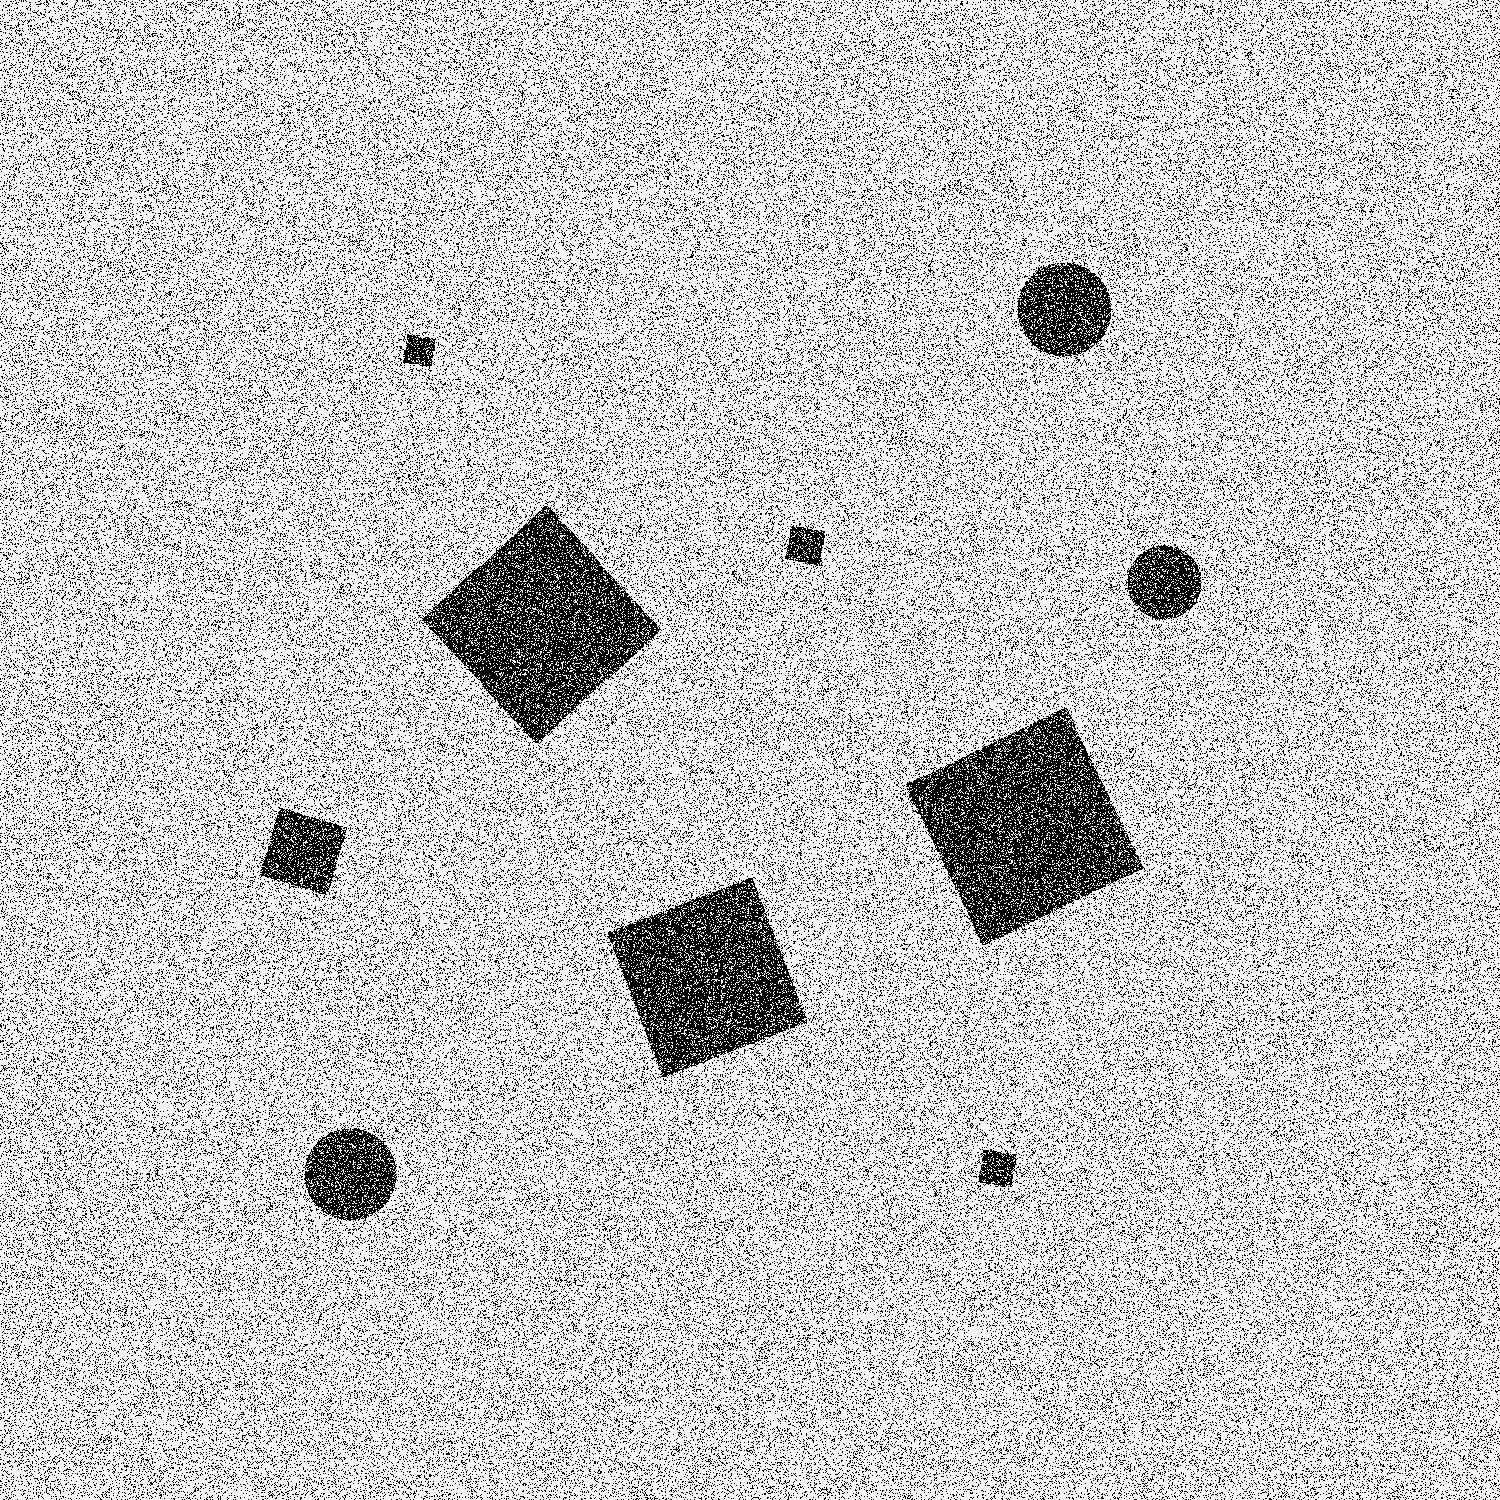
\includegraphics[scale = 0.2]{pic/178E3-hard-2.png} \end{center}

    $1000 \leq n \leq 2000$ 
\subsubsection{算法}
\label{sec-10-6-2}

    由于每个点 20\% 的几率变成颜色相反的点这个条件太可怕了,我们考虑将整个图形模糊一下。一种方法是加权平均数,也就是每个点取相邻点的加权平均数,然后再取个整。权的话,我们可以模仿高斯模糊\footnote{http://zh.wikipedia.org/wiki/高斯模糊
 }。我取了周围 9 个点,然后将整个图模糊 10 次。

    经过模糊处理后,我们得到的图中,不仅有圆/正方形,还有若干个形状未知的小块。小块的处理很简单,题目保证圆/正方形的直径不小于 15 个像素,我们判断如果块的大小小于某个值(我取 200 ),就把这个小块的颜色全部取反。

    经过前两步的处理,我们得到的图像如下\footnote{用 Python 的 PIL 库生成。\href{http://www.pythonware.com/products/pil/}{http://www.pythonware.com/products/pil/}
 }:

\begin{center}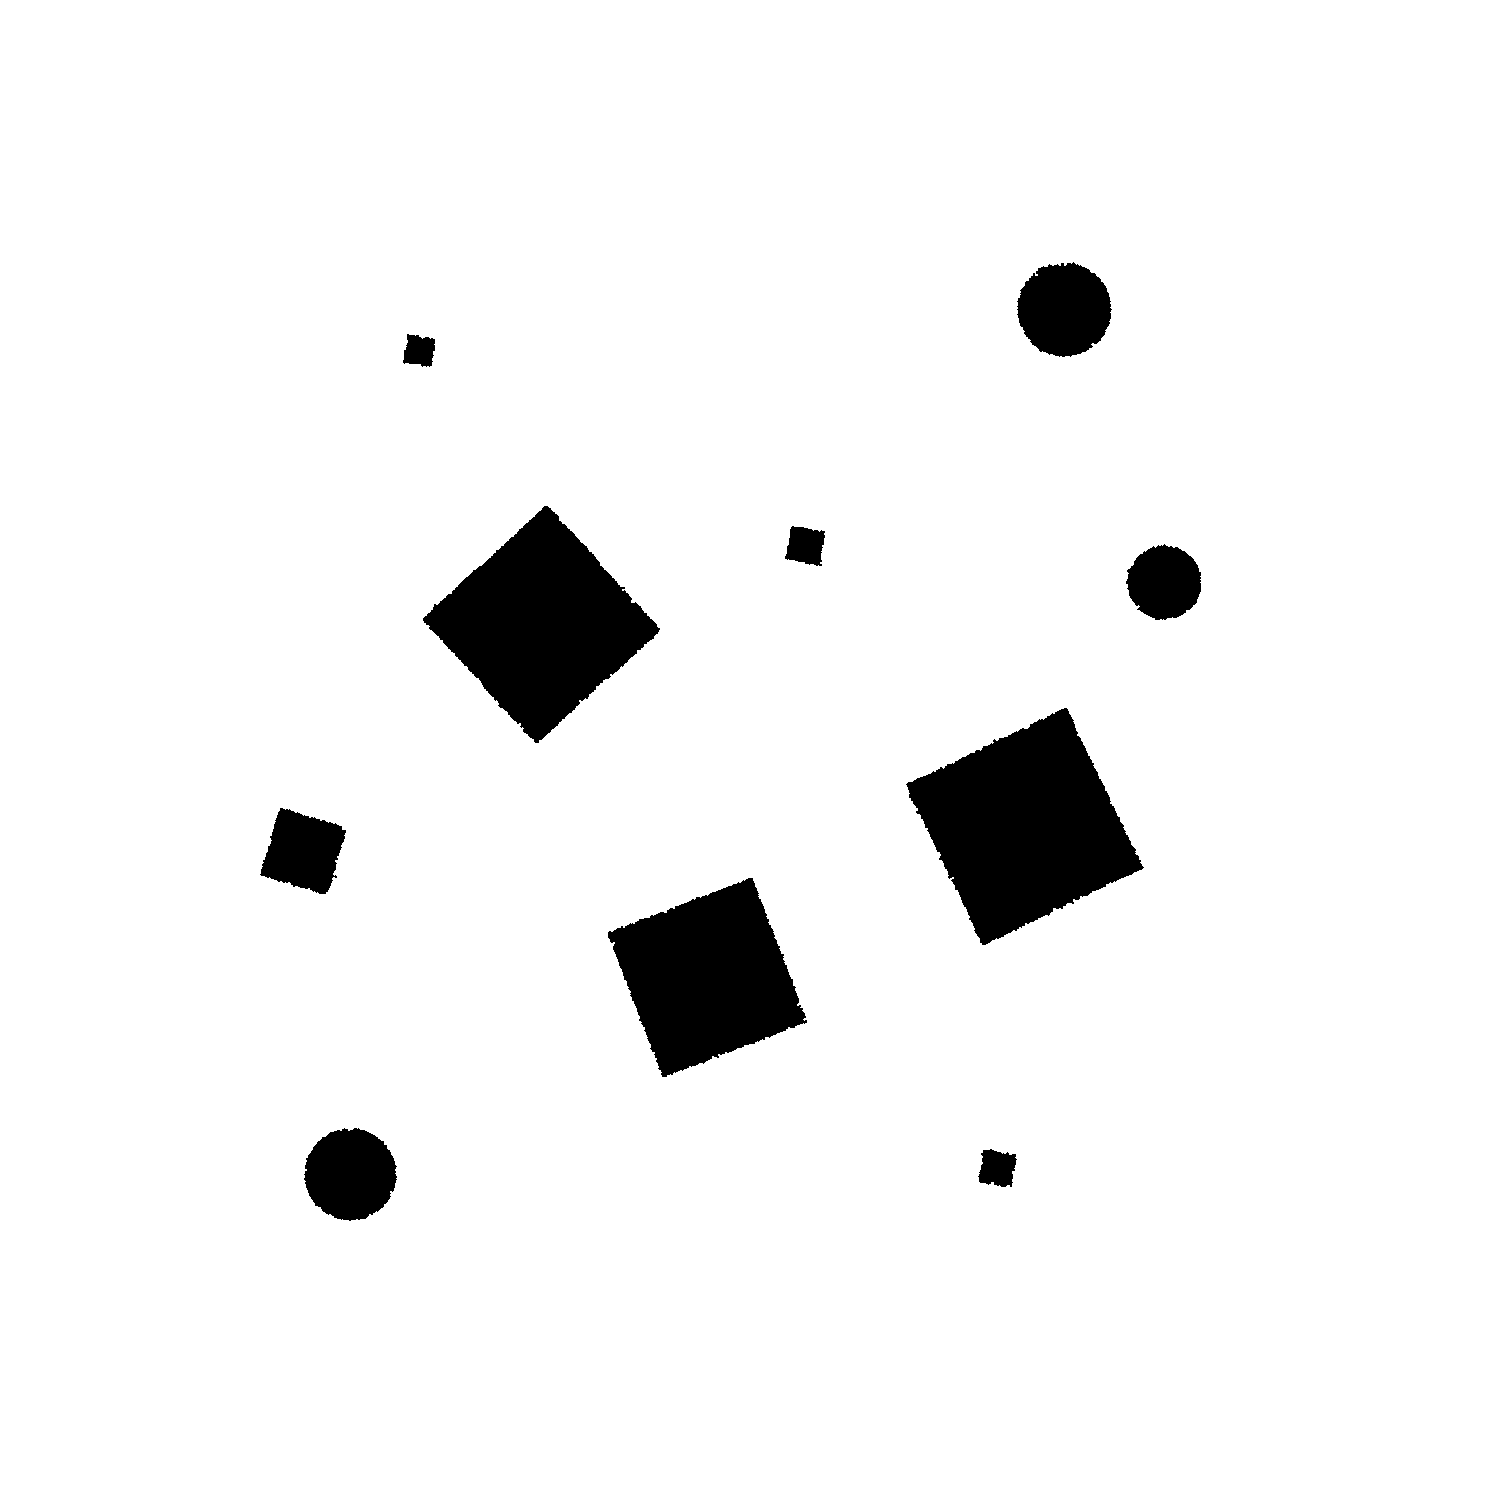
\includegraphics[scale = 0.2]{pic/178E3-hard-2-show.png}\end{center}

    没有了干扰点了。对于每个块,只需暴力 BFS 出块的大小 $n$ 以及到中心点的最大距离 $r$ ,对于圆我们有 $n \sim \pi r^2$ ,对于正方形我们有 $n \sim 2 r^2$ ,所以我们取个中,判断 $n$ 与 $2.5 r^2$ 的大小关系即可。
\subsection{180B  Divisibility Rules}
\label{sec-10-7}
\subsubsection{题意}
\label{sec-10-7-1}

    在 10 进制下, $n \vert d$ 的条件有以下几类:
\begin{enumerate}
\item $d = 2, 4, 5, 8, 10$ 时,检查最后几位是否能整除 $d$ 即可。这种 $d$ 称作 $2-type$ 。
\item $d = 3, 9$ 时,检查所有数位的和是否能整出 $d$ 即可。这种 $d$ 称作 $3-type$ 。
\item $d = 11$ 时,检查奇数位的和减去偶数位的和是否能整除 $d$ 即可。这种 $d$ 称作 $11-type$ 。
\item $d = 6$ 时,检查以上若干个条件即可。这种 $d$ 称作 $6-type$ 。
\item $d = 7$ 时,没有快速的方法。这种 $d$ 称作 $7-type$ 。
\end{enumerate}
    求 $b$ 进制下 $d$ 属于哪一类。如果同时属于 $3-type$ 和 $11-type$ ,输出 $3-type$ 。如果是 $2-type$ ,输出要检查几位。

    $2 \leq b, d \leq 100$
\subsubsection{算法}
\label{sec-10-7-2}

    一个一个枚举过去即可。
\begin{enumerate}
\item $2-type$ 的条件: $d$ 只含有 $b$ 以外的质因子,每次 $d$ 除以 $gcd (d, b)$ ,除几次变成 1 就要检查几位。
\item $3-type$ 的条件: $d \vert (b - 1)$
\item $11-type$ 的条件:$d \vert (b + 1)$
\item $6-type$ 的条件: $\frac{d}{gcd (d, b^2 - 1)}$ 是 $2-type$ 。
\item 否则就是 $7-type$ 。
\end{enumerate}
\subsection{185D  Visit of the Great}
\label{sec-10-8}
\subsubsection{题意}
\label{sec-10-8-1}

    给定 $k, l, r, p$ ,求
    $$LCM (k^{2^l}, k^{2^{l + 1}}, \dots, k^{2^{r}}) \mod{p}$$

    $k \leq 10^6, 1 \leq l \leq r \leq 10^18, 1 \leq p \leq 10^9$ 且 $p$ 为质数,测试数据组数不超过 $10^5$ 。
\subsubsection{算法}
\label{sec-10-8-2}

    如果 $p = 2$ ,则 $k$ 为奇数时答案为 0 , $k$ 为偶数时答案为 1 。

\begin{theorem}
  若 $a \neq b$ ,则 
  $$gcd (k^{2^a} + 1, k^{2^b} + 1) = \begin{cases} 2 & \text{if} k \equiv 1 \mod{2} \\ 1 & \text{otherwise}\end{cases}$$
\end{theorem}
\begin{proof}
  不妨令 $a < b$ ,有
  $$
  (k^{2^a} - 1)(k^{2^a} + 1)(k^{2^{a + 1}} + 1) \dots (k^{2^{b - 1}} + 1) = k^{2^b} - 1
  $$
  也就是 $$k^{2^b} + 1 \equiv 2 \mod{k^{2^a} + 1}$$
  然后结论显然了。
\end{proof}

    所以,当 $k$ 为奇数时,答案为 $\frac{1}{2^{r - l}} \Pi_{i = l}^r (k^{2^i} + 1)$ ,否则答案为 $\Pi_{i = l}^r (k^{2^i} + 1)$ 。我们只需求出这个 $\Pi$ 即可。

    易得 $$\Pi_{i = l}^r (k^{2^i} + 1) = \frac{k^{2^{r + 1}} - 1}{k^{2^l} - 1}$$ 。如果 $k^{2^l} \not\equiv 1 \mod{p}$ ,直接上逆元即可。如果 $k^{2^l} - 1 \equiv 1 \mod{p}$ ,则 $k^{2^l} + 1 \equiv 2 \mod{p}$ , $Pi$ 即为 $2^{r - l + 1}$ 。

    时间复杂度为 $O(T \log rp)$ 。
\subsection{187D  BRT Contract}
\label{sec-10-9}
\subsubsection{题意}
\label{sec-10-9-1}

    已知从起点开往终点,中间经过 $n$ 个红绿灯。所有的红绿灯都是先亮 $G$ 单位时间的绿灯,再亮 $R$ 单位时间的红灯。出发时所有的灯都恰好由红转绿。已知 $l_i$ 表示从第 $i - 1$ 个红绿灯到第 $i$ 个红绿灯的距离,汽车行驶速度是 1 单位距离/单位时间。遇到红灯必须等,绿灯才可以走。有 $Q$ 辆车,到达起点的时间为 $f_i$ ,求每辆车到达终点的时间。

    $1 \leq l_i \leq 10^9, n, Q \leq 10^5, 2 \leq G + R \leq 10^9$
\subsubsection{算法}
\label{sec-10-9-2}

    令 $rem_i$ 表示在 0 时刻到达第 $i$ 个红绿灯后,到达终点还需多少时间, $next_i$ 表示在 0 时刻到达第 $i$ 个红绿灯后,下一个遇到的红灯是哪一个。易知 $rem_i = rem_{next_i} + (G + R)\ceil{\frac{dist_{next_i} - dist_i}{G + R}}$ ,其中 $dist_i$ 表示起点到第 $i$ 个红绿灯的距离。所以,我们只需快速求出 $next_i$ 即可。

    考虑如何求 $next_i$ 。 $next_i$ 一定是最小的满足 $dist_j - dist_i \mod{G + R} \in [G, G + R)$ 的 $j$ ,也就是查询满足 $dist_j \in [G + dist[i] \mod{G + R}, dist[i] \mod{G + R})$ 的最小的 $j$ 。我们从后往前依次求 $next_i$ ,顺便维护一棵线段树,每次在 $dist_i$ 这个位置插入 $i$ ,求 $next_i$ 的话直接用线段树进行区间查询即可。

    至于每次查询,我们用类似的思想,每次找到第一个遇到的红灯即可。还是用线段树。

    时间复杂度 $O((n + Q) \log n)$ 。
\section{Volume XI}
\label{sec-11}
\subsection{176E  Archaeology}
\label{sec-11-1}

   \ref{176E}
\subsubsection{题意}
\label{sec-11-1-1}

    给定大小为 $n$ 的一棵边权树,维护以下操作:
\begin{enumerate}
\item 激活一个点
\item 冻结一个点
\item 询问这若干个点的 MST 的权值。
\end{enumerate}

    $n, Q \leq 10^5$ 
\subsubsection{算法}
\label{sec-11-1-2}

    不妨以任意一个点为根,易知每次询问的答案为:所有激活点到根的路径的并的权值和 - 激活点的个数 $\times$ 所有激活点的公共 LCA 到根的距离。
    所以,我们同时维护这三个量即可。

    如何求所有激活点到根的路径的并的权值和呢?有一个很经典的做法: dfs 这棵树,遇到一个激活点,就把这个激活点和最后一次遇到的激活点的 LCA 到这个激活点的距离加入答案;如果是第一次遇到激活点,那么直接把这个点到根的距离加入答案。正确性显然。这样做是可以维护的。我们求出每个点在 dfs 中被访问的顺序,以此为关键字维护一个 set ,每次加入一个点的话只有相邻的两个点会对答案造成影响,于是重新维护这几个点的贡献即可。

    如何维护所有激活点的公共 LCA 呢?如果有 dfs 序 ,那么公共 LCA 就是 dfs 序中第一个激活点与最后一个激活点的 LCA 。正确性也显然。

    时间复杂度为 $O(n + Q \times LCA (u, v))$ 。其中 $LCA (u, v)$ 表示查询 $u$ 、 $v$ 两点的 LCA 的复杂度。用倍增/树链剖分可以做到 $O(\log n)$ 。
\subsection{196D  The Next Good String}
\label{sec-11-2}
\subsubsection{题意}
\label{sec-11-2-1}

\begin{definition}
    一个字符串 $S$ 被称为好串,当且仅当 $S$ 不存在一个长度不小于 $d$ 的子串是回文串。
\end{definition}
给定一个字符串 $S$ ,求一个长度为 $|S|$ 、字典序严格比 $S$ 大的好串。

$|S| \leq 5 \times 10^5$
\subsubsection{算法}
\label{sec-11-2-2}

易知,只要不存在长度为 $d$ 或者 $d + 1$ 的子串是回文串,那么这个字符串就是回文串。

然后就是贪心:每次将最靠前的一个长度为 $d$ 或者 $d + 1$ 的回文子串改掉。我们可以用 dfs 来实现这个过程,实时维护 hash 来判断是否是回文串即可。

时间复杂度 $O(n)$ 。
    
\subsection{198E  Gripping Story}
\label{sec-11-3}
\subsubsection{题意}
\label{sec-11-3-1}

    二维平面上有 $n$ 块磁铁,每块磁铁有三个属性 $m, p, r$ ,分别表示这块磁铁的质量、磁力、磁力半径。你在一个点 $(x, y)$ ,有一块磁力半径为 $r$ 磁力为 $p$ 的磁铁,现在需要将磁铁尽量多地吸过来。你能够吸入一块磁铁 $i$ 的条件是,你已有一块磁铁 $j$ ,使得 $p_j \geq m_i, r_j \geq dist (i, j)$ ,这里的距离是指欧几里得距离。求最多能吸引多少块磁铁。

    $n \leq 250000, |x|, |y|, p, r \leq 10^9$ 
\subsubsection{算法}
\label{sec-11-3-2}

    很容易可以看出贪心是可行的:每次用某块已有的磁铁吸入所有能吸入的磁铁,直至不能为止。暴力实现 $O(n^2)$ 会 TLE ,我们用数据结构优化即可。我的方法是按距离从小到大排序,维护一个树状数组,树状数组里的每个元素是一个若干个磁铁的集合,用 set 暴力维护,排序的关键字是这块磁铁的质量。那么每次我们在树状数组里面的 set 查,如果质量最小的磁铁能够被吸入,那就吸入,然后在树状数组中删除这个元素。

    时间复杂度为 $O(n \log^2 n)$ 。
\subsection{200E  Tractor College}
\label{sec-11-4}
\subsubsection{题意}
\label{sec-11-4-1}

    给定四个非负整数 $c_3, c_4, c_5, S$ 要求 $k_3, k_4, k_5$ ,满足:
    \begin{displaymath}
    \begin{cases}
    \label{ref:200E-1} 0 \leq k_3 \leq k_4 \leq k_5 \\
    \label{ref:200E-2} c_3 k_3 + c_4 k_4 + c_5 k_5 = S \\
    \label{ref:200E-3} |c_3 k_3 - c_4 k_4| +|c_4 k_4 - c_5 k_5| \text{最小} \\
    \end{cases}
    \end{displaymath}

    $c_3 + c_4 + c_5 \leq 10^5, S \leq 10^5$
\subsubsection{算法}
\label{sec-11-4-2}

    不妨枚举 $k_4$ 。根据 \ref{ref:200E-2} 可以由拓展欧几里得求出一组解 $k_3 = a, k_5 = b$ ,可以知道对于每组解,都有 $k_3 = a + c_3 t, k_5 = b - c_5 t, t \in Z$ 。根据 \ref{ref:20E-1} 可以知道 $t$ 的范围,易知 \ref{ref:200E-3} 关于 $t$ 是单调的,三分 $t$ 即可。

    时间复杂度 $O(S \log (c_3 + c_4 +c_5))$ 。
 
\subsection{200A  Cinema}
\label{sec-11-5}
\subsubsection{题意}
\label{sec-11-5-1}

    给定一个 $n \times m$ 的棋盘,初始时全部是白的。现在要往棋盘上染色,每次给定一个坐标 $(x, y)$ ,要求找到满足以下条件的格子:
\begin{enumerate}
\item \label{ref:200A-1} 距离 $(x, y)$ 最小。此处距离指曼哈顿距离。
\item \label{ref:200A-2} 在满足 \ref{ref:200A-1} 的前提下 $x$ 坐标尽量小。
\item 在满足 \ref{ref:200A-2} 的前提下 $y$ 坐标尽量小。
\end{enumerate}
    并把它染成黑色。

    $n, m \leq 2000, k \leq \min(10^5, nm)$
\subsubsection{算法}
\label{sec-11-5-2}

我们把棋盘旋转 $45^\circ$ ,用二维树状数组维护二维前缀和。每次找格子时,二分曼哈顿距离,用树状数组检验是否有空,如果有的话暴力从小到大枚举 $x$ 坐标即可。

时间复杂度 $O(k \log^3 n)$ 。

再介绍另一个算法。对于每个 $x$ ,我们维护每个点上下第一个没有被删除的点是哪个。对于每次询问,我们暴力枚举横坐标,如果当前横坐标与目标横坐标差大于已有的最优解就直接 break ,否则利用上下的点更新答案。这样的最坏情况是 $O(Kn)$ 的。如果我们保证 $n > m$ ,那么可以证明,这样做的最坏情况是 $O(\min(sqrt(K), m)$ 的。
\subsection{201E  Thoroughly Bureaucratic Organization}
\label{sec-11-6}
\subsubsection{题意}
\label{sec-11-6-1}

    有一个 $n$ 的排列,你一次可以询问不超过 $m$ 个位置的值,但是返回的结果是乱序的,也就是返回的若干个值恰好是这若干个位置对应的值,但是顺序不一定相同。求最优策略下至少要询问多少次才可以确定原排列。

    $n, m \leq 10^5$ ,数据组数不超过 1000 组。
\subsubsection{算法}
\label{sec-11-6-2}

    换个思路:给定 $k, m$ ,求 $f(k, m)$ 表示询问 $k$ 次,每次不超过 $m$ 个位置的值,最大能确定的 $n$ 。如果能够快速求出 $f(k, m)$ ,那么我们就可以二分答案了。如何求 $f$ 呢?贪心。令 $a_{i, j}$ 表示数字 $i$ 在第 $j$ 次询问中是否出现,题目中的限制为 $\sum_{i} a_{i, j} \leq m$ ,而 $f (k, m)$ 则表示不同的 $a_i$ 的个数。可以证明,只要 $\sum_{i, j} a_{i, j} \leq km$ ,那么就一定可以找出一个方案使得 $\sum_{i} a^\prime_{i, j} \leq m$ 且 $a^\prime$ 中不同 $a^\prime_i$ 的个数与 $a$ 中的一样多。

    于是问题转换为:
\begin{problem}
  已知 $\sum_{1 \leq j \leq k} a_{i, j} \leq km$ ,求最多有多少个不同的 $a_i$ 。
\end{problem}
    贪心的想,将 $a_i$ 按照 1 的个数排序后,一定是所有放 0 个 1 ,然后是所有放 1 个 1 的,然后是所有放 2 个 1 的,直到没有足够的 1 为止。易知每次做的复杂度是 $O(\log n)$ 的。

    所以整体时间复杂度是 $O(T \log^2 n)$ 。
\subsection{201D  Brand New Problem}
\label{sec-11-7}
\subsubsection{题意}
\label{sec-11-7-1}

    给定一个长为 $n$ 的无重的字符串序列 $S$ ,以及 $m$ 个字符串序列 $T_{1 \dots m}$ ,要求找到一个逆序对数最少的 $1 - n$ 的排列 $p$ ,使得序列 $S_{p_i}$ 是 $T_j$ 的子序列。

    $n \leq 15, 1 \leq m \leq 10, \sum |T_i| \leq 5 \times 10^5$ 
\subsubsection{算法}
\label{sec-11-7-2}

    暴力 dp $f_{i, j, S}$ 表示 $T_i$ 的前 $j$ 位中排列出现了 $S$ 这个集合的最小逆序对数是肯定会 T 的,我们要想办法优化。

    一种优化方式是:令 $f_{i, S, inv}$ 表示 $T_i$ 中,出现了 $S$ 这个集合且已知逆序对数恰好为 $inv$ 时,最少要匹配到 $T_i$ 的第几个字符串。转移就是枚举下一个字符串是什么,预处理出 $T_i$ 的第 $j$ 个位置开始第一次出现 $x$ 的位置,就可以枚举后 $O(1)$ 转移了。

    时间复杂度 $O(n^3 2^n + n \sum |T_i|$ 。
\subsection{204E  Little Elephant and Strings}
\label{sec-11-8}
\subsubsection{题意}
\label{sec-11-8-1}

    给定 $n$ 个串 \$S\_{}{1 \dots n}\$,对于每个串,求出有多少个子串,使得这个子串至少在 $n$ 个串中的 $k$ 个串中出现过。

    $n, k \leq 10^5, \sum |S_i| \leq 10^5$
\subsubsection{算法}
\label{sec-11-8-2}

    我们对这 $n$ 个串构出一棵 trie ,然后求出这个 trie 的后缀自动机,顺便可以构出这个 trie 的逆序的后缀树。对于每个串 $S_i$ ,在后缀树上有若干个节点,那么后缀树上的一个节点所代表的字符串在 $S_i$ 中出现过的条件是:这个节点在与 $S_i$ 相关的若干个节点到根的路径的并上。那么对于每个串 $S_i$ ,我们把与 $S_i$ 相关的若干个节点到根的路径的并上的每个节点的计数器都加一,那么一个节点所代表的串在至少 $k$ 个串中出现的条件就是它的计数器不小于 $k$ 。我们再记录每个节点到根的路径上,第一个计数器不小于 $k$ 的节点是哪个,那么就可以得到这个节点所代表的串有多少个前缀在至少 $k$ 个串中出现过。依次枚举 $S_i$ 的后缀,加起来即可。

    现在还剩下一个问题,如何把与 $S_i$ 相关的若干个节点到根的路径的并上的每个节点的计数器都加一。这是个很经典的问题,可以参考 \ref{176E} 的方法。
\subsection{207B1 Military Trainings (20 points)}
\label{sec-11-9}
\subsubsection{题意}
\label{sec-11-9-1}

给定一个长为 $n$ 的序列 $a_i$ ,规定点 $i$ 一次跳跃能到点 $j$ 的条件是: $i \geq j - a_j$ ,现在有 $n$ 次操作,每次操作如下:
\begin{enumerate}
\item 询问从第一个点到最后一个点至少要多少次跳跃
\item 将 $a$ 的最后一个元素删除,并插入到 $a$ 最前面
\end{enumerate}

$n, a_i \leq 250000$
\subsubsection{算法}
\label{sec-11-9-2}

我们先将 $a$ 数组粘贴在自身后面,那么原题变为: $n$ 次询问,每次询问 $i + 1$ 到 $i + n$ 至少要几次跳跃。

令 $f_{i, j}$ 表示起始点至少要在 $f_{i, j}$ 才能在 $2^j$ 步内跳到 $i$ 处。可以得到 $f_{i, j}$ 的递推式为
$$f_{i, j} = \begin{cases} i - a_i + 1 & j = 1 \\ \min_{t = f_{i - 1, j - 1}^i} f_{t, j - 1} \text{otherwise} \end{cases}$$
易知预处理时间复杂度为 $O(n \log^2 n)$ 。

考虑每次查询从 $s$ 跳到 $t$ 的最少次数。我们可以二分,然后利用 $f$ 判断是否可以到达,这样复杂度是 $O(n \log^2 n)$ 的,当然,直接在 $f$ 上走也是可以的。我们从 $\floor{\log_2 n}$ 开始枚举 $j$ ,如果 $f_{t, j} \leq s$ ,我们就可以更新答案,否则就令 $t = f_{t, j}$ 。

时间复杂度 $O(n \log^2 n)$ 。
\section{Volume XII}
\label{sec-12}
\subsection{207A2 Beaver's Calculator (30 points)}
\label{sec-12-1}
\subsubsection{题意}
\label{sec-12-1-1}

给定 $n$ 个序列,第 $i$ 个序列长度为 $k_i$ 。现在要求将这 $k$ 个序列归并成一个序列,使得新序列 $a$ 中,满足 $a_i > a_{i + 1} \quad (i \leq n)$ 的 $i$ 尽量少。

$2 \leq n \leq 5000, 2 \leq k \leq 5000$
\subsubsection{算法}
\label{sec-12-1-2}

贪心即可。每次取不小于上次的最小的数。如果不存在,取最小的即可。这样做是 $O(\sum k \log n)$ 的,可以过 CodeForces 上的数据。

研究这个算法,可以考虑给每个序列分层。对于一个序列 $a$ ,如果 $a_i \leq a_{i + 1}$ ,那么 $a_i$ 和 $a_{i + 1}$ 的就可以分在同一层,否则就不能。可以知道,对于同一层的所有数来说,一定存在一种方法使得不存在 $a_i > a_{i + 1}$ ,因为这是对若干个有序数组进行归并,而不同层的至少会对答案贡献 1 ,所以最后的答案就是这若干个数组中,层数最多的数组的层数。这样我们只需分开统计每一个数组的层数就可以了。

时间复杂度 $O(\sum k)$ 。
\subsection{167D  Wizards and Roads}
\label{sec-12-2}
\subsubsection{题意}
\label{sec-12-2-1}
\subsubsection{算法}
\label{sec-12-2-2}
\subsection{209C  Trails and Glades}
\label{sec-12-3}
\subsubsection{题意}
\label{sec-12-3-1}

    给定一个无向图,要求添加尽量少的边,使得从 1 开始能够遍历所有的边恰好一次并回到 1 。

    $n, m \leq 10^6$
\subsubsection{算法}
\label{sec-12-3-2}

    这个题的要求为:
\begin{enumerate}
\item 每个点的度数为偶数
\item 只存在一个连通块,且 1 在这个连通块中。
\end{enumerate}

    我们用并查集处理出一开始有多少个连通块,以及每个连通块内度数为奇的点的个数,如果 1 没有边,那么 1 也应该算一个连通块。把所有连通块按照奇度数点的个数从小到大排序,每次我们可以在两个连通块之间添加一条边,可以得到一个新的连通块。如果一个连通块有奇度数点,那么这条边就应该连在某个奇度数点上,否则只能连在某个偶度数点上。贪心的想,我们应该按照连通块中奇度数点的个数从大到小合并所有的块,到最后只剩下一个大块时再添加若干条边即可。

    时间复杂度 $O(n \log n + m \alpha (n))$ 。
\subsection{212B  Polycarpus is Looking for Good Substrings}
\label{sec-12-4}
\subsubsection{题意}
\label{sec-12-4-1}

给定一个长为 $n$ 的只包含小写字母的字符串 $S$ ,再给定 $m$ 组询问,每次给定一个字符串集合 $C$ ,询问 $S$ 中有多少个极大子串 $T$ ,使得 $T$ 中的每个字符都在 $C$ 中出现过, $C$ 中的每个字符都在 $T$ 中出现过。

$n \leq 10^6, m \leq 10^4$
\subsubsection{算法}
\label{sec-12-4-2}

由于只包含小写字母,我们可以得到:
\begin{theorem}
  至多有 $26n$ 个不同的极大的字符串。
\end{theorem}

于是我们只要枚举出每个极大的字符串即可。我们记录每个位置之后第一个字符 $c$ 出现位置。对于位置 $i$ ,我们将 \texttt{a} 到 \texttt{c} 按照第一次出现的位置排序,从前到后扫描即可。

时间复杂度 O(26n) 。
\subsection{212D  Cutting a Fence}
\label{sec-12-5}
\subsubsection{题意}
\label{sec-12-5-1}

给定一个长为 $n$ 的序列 $a_{1 \dots n}$ ,有 $m$ 个询问,每次给定一个 $k$ ,求 $\min\{a_{i + 1} \dots a_{i + k}\} (0 \leq i \leq n - k)$ 的期望值。

$n \leq 10^6, m \leq 10^6$
\subsubsection{算法}
\label{sec-12-5-2}

由于数据组数特别多,我们可以考虑将所有的答案全部处理出来。

考虑一个数 $i$ ,到左边第一个比 $a_i$ 大的数的距离为 $L_i$ ,到右边第一个比 $a_i$ 大的数的距离为 $R_i$ 。这两个值可以通过维护一个栈在 $O(n)$ 的时间内求出来。截下来我们在二维平面上画一个矩形,左下角为 (0, 0) ,右上角为 $(L_i, R_i)$ ,然后给这个矩形内部的整点全部加上 $a_i$ ,那么对于一个询问 $k$ ,答案就是要得到直线 $x + y = k - 1$ 经过的整点的权值和。考虑一个矩形对所有 $k$ 的影响,可以发现这是对所有 1 到 $\min(L_i, R_i)$ 的数依次加上 $a_i$ 到 $a_i \min(L_i, R_i)$ ,对于 $\min(L_i, R_i) + 1$ 到 $\max(L_i, R_i)$ 内的所有的 $k$ 加上 $a_i (\min(L_i, R_i) + 1)$ ,对于 $\max(L_i, R_i) + 1$ 到 $L_i + R_i + 1$ 内的所有的 $k$ 依次加上 $a_i (\min(L_i, R_i) + 1)$ 到 $a_i$ 。差分两次,就可以在 $O(n)$ 的时间内得到所有的答案。

时间复杂度为 $O(n)$ 。
\subsection{212C  Cowboys}
\label{sec-12-6}
\subsubsection{题意}
\label{sec-12-6-1}

给定一个大小为 $n$ 的环,环上的每个点要么指向下一个点,要么指向上一个点。定义两个环之间的变换为:如果原环两个点互指,那么新环中两个点都不指向另一个。已知变换之后的环,求有多少种不同的原环使其变换之后为新环。

$n \leq 100$
\subsubsection{算法}
\label{sec-12-6-2}

如果新环中两个点互指,那么原环中两个点一定不互指。如果新环中两个点都不指对方,那么原图中两个点有可能互指。

于是我们将题目进行变换:将原环中相邻两个点看成是一个对,有些对可以取反(原环这一对 \textbf{可能} 互指),然后规定若干相邻对中至少有一个必须取反(原环中这一对一定不互指),求方案数。可以发现,变换后的题目所构的图可以被拆成若干条链,链与链之间是不相关的,我们只需对每条链单独处理即可。如果是一个环,答案就是 $fib_{n + 1} + fib_{n - 1}$ 。

对于一条长度为 $n$ 的链,如果首尾均无限制,那么方案数为 $fib_{n + 1}$ ,即第 $n + 2$ 个 $fibonacci$ 数。如果首/尾有限制,去掉首/尾即可。

时间复杂度为 $O(n)$ 。
\subsection{213E  Two Permutations}
\label{sec-12-7}
\subsubsection{题意}
\label{sec-12-7-1}

给定两个长度分别为 $n$ 和 $m$ 的排列 $S$ 和 $T$ ,求有多少个 $k$ ,使得 $\{S_i + k\}$ 是 $T$ 的子序列。

$n, m \leq 200000$
\subsubsection{算法}
\label{sec-12-7-2}

用线段树可以很方便的维护一个序列的 hash 。我们查询 $n - m$ 次,每次查询 $\{S_i + k\}$ 的 hash 即可。对于 $k$ 与 $k + 1$ ,我们只需在线段树中删除 $k - n$ ,加入 $k$ 即可。

时间复杂度 $O(m \log m)$ 。
\subsection{217C  Formurosa}
\label{sec-12-8}
\subsubsection{题意}
\label{sec-12-8-1}

有 $n$ 不全相同的 0/1 变量 $x_i$ ,给定一个多元 0/1 函数 $f$ ,问是否能利用 $f$ 求出所有的 $x$ 。

$f$ 由一个字符串 $s$ 描述, $s$ 的语法为: $s = 0 | 1 | ? | (s ^ s) | (s | s) | (s \& s)$ 其中 \texttt{?} 表示函数的参数。

$n \leq 10^6, |s| \leq 10^6$
\subsubsection{算法}
\label{sec-12-8-2}

我们先对 $s$ 进行字符串处理,求出这个表达式树。分析在怎样一种情况下可以求出所有变量的值。可以得到如下结论:

\begin{theorem}
能求出所有的 $x$ 的充要条件是存在一个 0/1 序列 $S$ 使得 $f(S) \neq f(-S)$ ,其中 $-S$ 表示把 $S$ 中的每个元素取反。
\end{theorem}
\begin{proof}
如果不存在这样一个序列的话,我们把所有 $x$ 取反,那么所有的函数值都不会变,无法求出所有的 $x$ 。

如果存在这样一个序列,那么我们枚举两个变量 $x_a, x_b$ ,先把 $S$ 中所有的 0 替换成 $x_a$ ,1 替换成 $x_b$ ,求 $f(S)$ ,再把 $S$ 中所有的 0 替换成 $x_b$ , 1 替换成 $x_a$ ,求 $f(S)$ ,如果两个值不一样,那么我们可以确定出 $x_a, x_b$ 各为多少。由于 0/1 至少出现 1 次,我们因此每个数我们都可以确定出来。
\end{proof}

所以我们要做的就是判断有没有这么序列 $S$ 存在。这可以通过 dp 来解决。令 $f_{i, j, k}$ 表示对于子树 $i$ 所表示的函数 $F_i$ ,是否存在一个序列 $S$ 使得 $F_i (S) = j, F_i (-S) = k$ 。转移时枚举两个孩子即可。

时间复杂度 $O(|S|)$ 。
\subsection{229E  Gifts}
\label{sec-12-9}
\subsubsection{题意}
\label{sec-12-9-1}
\subsubsection{算法}
\label{sec-12-9-2}

\end{document}